\documentclass[journal]{IEEEtran}

\usepackage{amsmath,amssymb}
\usepackage{graphicx}
\usepackage{booktabs}
\usepackage{siunitx}
\usepackage{url}
\usepackage{xcolor}
\usepackage{array}
\usepackage{multirow}
\usepackage{balance}

\newcommand{\nside}{N_{\mathrm{side}}}
\newcommand{\level}{\ell}
\newcommand{\hpix}{\mathrm{HEALPix}}
\newcommand{\Rearth}{R_{\oplus}}
\newcommand{\todo}[1]{\textcolor{red}{[TODO: #1]}}

\begin{document}

\title{Rate--Distortion Trade-offs of an Oversampled HEALPix Carrier Grid for Sentinel-2 Imagery}

\author{
Jean-Marc Delouis\textsuperscript{1},
Tina Odaka\textsuperscript{2},
Benoit Bovy\textsuperscript{3},
Etienne Cap\textsuperscript{4},
Thomas Davison\textsuperscript{5},
Anne Fouilloux\textsuperscript{6},
Camille Gueguen\textsuperscript{7},
Alexander Kmoch\textsuperscript{8},
Justus Magin\textsuperscript{9},
Pablo Richard\textsuperscript{10},
and Vincent Dumoulin\textsuperscript{11}%
\thanks{\textsuperscript{1}LOPS UMR 6523,
CNRS--IFREMER--IRD--Univ. Brest--IUEM, Plouzané, France.
Corresponding author: jean.marc.delouis@ifremer.fr. ORCID: 0000-0002-0713-1658.}%
\thanks{\textsuperscript{2}LOPS UMR 6523,
CNRS--IFREMER--IRD--Univ. Brest--IUEM, Plouzané, France.
Email: Tina.Odaka@ifremer.fr. ORCID: 0000-0002-1500-0156.}%
\thanks{\textsuperscript{3}GEORODE, Liège, Belgium.
Email: bbovy@georode.com. ORCID: 0009-0001-4011-3574.}%
\thanks{\textsuperscript{4}LOPS UMR 6523,
CNRS--IFREMER--IRD--Univ. Brest--IUEM, Plouzané, France.
Email: Etienne.Cap@ifremer.fr. ORCID: 0009-0007-0360-0692.}%
\thanks{\textsuperscript{5}European Space Agency (ESA)---ESRIN, Frascati, Italy.
Email: Thomas.Davison@esa.int. ORCID: 0000-0002-0917-4256.}%
\thanks{\textsuperscript{6}LifeWatch ERIC, Seville, Spain.
Email: anne.fouilloux@lifewatch.eu. ORCID: 0000-0002-1784-2920.}%
\thanks{\textsuperscript{7}LOPS UMR 6523,
CNRS--IFREMER--IRD--Univ. Brest--IUEM, Plouzané, France.
Email: camille.gueguen@ifremer.fr. ORCID: 0009-0008-3748-9395.}%
\thanks{\textsuperscript{8}University of Tartu,
Institute of Ecology and Earth Sciences,
Landscape Geoinformatics Lab, Tartu, Estonia.
Email: alexander.kmoch@ut.ee. ORCID: 0000-0003-4386-4450.}%
\thanks{\textsuperscript{9}LOPS UMR 6523,
CNRS--IFREMER--IRD--Univ. Brest--IUEM, Plouzané, France.
Email: Justus.Magin@ifremer.fr. ORCID: 0000-0002-4254-8002.}%
\thanks{\textsuperscript{10}Pablo Richard EI, Paris, France.
Email: pablorichard@hotmail.fr. ORCID: 0000-0002-5441-8213.}%
\thanks{\textsuperscript{11}European Space Agency (ESA)---ESRIN, Frascati, Italy.
Email: vincent.dumoulin@esa.int. ORCID: 0000-0001-5049-3817.}%
}

\markboth{IEEE Transactions on Geoscience and Remote Sensing,~Vol.~XX, No.~X, Month~2026}%
{Author \MakeLowercase{\textit{et al.}}: Rate--Distortion Trade-offs of an Oversampled HEALPix Carrier Grid}

\maketitle

\begin{abstract}
Hierarchical equal-area pixelizations such as HEALPix suit global Earth
observation, but their dyadic refinement restricts available resolutions to
powers-of-two steps. Sentinel-2's \SI{10}{m} bands fall between level 19
(\SI{12.4}{m}) and level 20 (\SI{6.2}{m}), so a level-20 carrier grid
oversamples them by a factor of about $2.58$ in per-cell area. We ask whether
that oversampling costs storage once compression and the overhead of native
tiling are both accounted for. On 40 Sentinel-2 L2A B04 regions spanning four
land-cover classes and latitudes from $43.5^\circ$S to $64.1^\circ$N, five
established general-purpose codecs are applied to level-20 chunks reshaped by
Morton de-interleaving, and to a native UTM square of equal nominal projected
area. Scored end-to-end against the same Sentinel-2 observation, over the
intersection of the two footprints, native UTM is the more efficient
representation at every target we can report: the uncompressed carrier tile
already differs from the observation by $4.0\times10^{-3}$ in median, about
$10\%$ of a scene's standard deviation, which places the tighter reconstruction
targets out of reach. We show that this floor belongs to the transfer-and-read
pair rather than to the grid: the nearest-cell read alone is a
\SI{2.1}{m} positional jitter that costs about $14\%$ of a field's standard
deviation on the imagery's own measured spectrum. Scored within each representation --- the operational
question of compressing an already-built HEALPix cube --- the verdict is
regime-dependent, native UTM leading at high fidelity (median ratios
$1.25$--$1.59$) and HEALPix at the tightest storage budget ($0.83$) under an
assumed $30\%$ granule overhead. We summarise this as a critical overhead
falling from $2.07$ to $1.08$ with the distortion target, and report both
measures rather than electing one.
\end{abstract}

\begin{IEEEkeywords}
Earth observation, HEALPix, discrete global grid systems, data compression, rate-distortion evaluation, JPEG~2000, JPEG~XL, ZFP, SZ, Sentinel-2, cloud-native geospatial data, remote sensing data management.
\end{IEEEkeywords}

\section{Introduction}
\label{sec:intro}
\IEEEPARstart{E}{arth} observation data archives are becoming ever larger, incorporating multiple sensors and resolutions, and are increasingly hosted in the cloud. Their effective scientific use relies on storage organizations that enable globally consistent spatial referencing, efficient local access, and scalable data chunking. Discrete Global Grid Systems (DGGS) meet these needs by dividing the Earth into discrete, hierarchically indexed cells that serve as a shared spatial reference framework for data storage, aggregation, and analysis~\cite{ogc_dggs,iso19170}. Prominent instances include H3~\cite{h3}, S2~\cite{s2geometry}, and HEALPix~\cite{gorski2005healpix}, which vary in terms of cell shape, refinement strategy, and how well they preserve area.

HEALPix was first designed for analyzing astronomical data on the sphere~\cite{gorski2005healpix}. It provides equal-area pixels, a dyadic hierarchical refinement structure, and a nested indexing system in which all descendants of a given pixel occupy a contiguous block of indices. These characteristics are equally appealing for Earth observation on the globe, but they impose a practical limitation: HEALPix resolution can only change by powers of two, so an instrument’s native ground sampling distance will almost never match a HEALPix level exactly. For example, the \SI{10}{m} bands of Sentinel-2 lie between level 19 (\SI{12.4}{m}, which is too coarse) and level 20 (\SI{6.2}{m}, which is geometrically safe but nominally oversamples the data).

This paper’s core question is whether such oversampling is truly expensive once realistic storage and compression are considered. The level-20 samples do not constitute independent observations at \SI{6.2}{m} resolution; instead, they form an overcomplete representation whose net information content is still limited by the original sensor response. If that redundancy can in fact be compressed effectively, then storing the data at level 20 and applying compression should be no more costly—and may even be cheaper—than maintaining the equivalent information in its native UTM grid. The latter, when distributed under a specific operational tiling layout such as Sentinel-2's MGRS granule scheme (including padding, overlaps, and per-tile metadata), can carry substantial storage overhead beyond the geographic area actually needed; this paper follows the common modeling convention of assuming such overhead to be around $30\%$, an operational-scenario assumption rather than a property of UTM as a coordinate reference system (Section~\ref{sec:overhead}).

This paper addresses the question in a direct, data-driven way, relying exclusively on established, independently maintained compression libraries and avoiding any HEALPix-specific implementation. The higher-resolution HEALPix level is handled strictly as a 2D raster—obtained by Morton/Z-order de-interleaving of the nested chunk—and then passed to standard codecs exactly as if it were a conventional image. The comparison is carried out over matched ground area on both grids: the HEALPix tile's centroid is used to extract an axis-aligned, equal-area square directly from the native UTM raster (Section~\ref{sec:utm_crop}), so that the UTM side always remains the untouched native product, never itself a resampled representation being compared against another resampled representation.

The contributions of this work are:
\begin{itemize}
    \item a storage--distortion formulation of the resolution mismatch between native Sentinel-2 sampling and the next finer HEALPix carrier level, including an explicit geometric accounting showing that level 20's $2.58\times$ nominal oversampling makes the raw, uncompressed HEALPix tile the \emph{larger} representation by a fixed factor of $\approx\!1.99$ under an assumed $\approx\!30\%$ Sentinel-2/MGRS granule-overhead scenario -- so that compression, not raw storage, is what must do the work of making HEALPix competitive;
    \item an equal-area, rate--distortion protocol that separates intrinsic grid compressibility from the overhead of that assumed operational layout via an explicit critical-overhead $\gamma_\star$ analysis, comparing HEALPix tiles against an axis-aligned native UTM square of identical nominal ground area (rather than a rotated-footprint bounding box, which we show silently inflates the UTM-side pixel count by roughly $2\times$), with matched reconstruction error and matched storage budget enforced via direct log--log interpolation over each codec's own sweep;
    \item an empirical evaluation across 40 Sentinel-2 regions -- four land-cover classes, latitudes $43.5^\circ$S to $64.1^\circ$N, hence both HEALPix cell-shape regimes, which lets us show that the storage verdict itself depends on where on the sphere a tile sits (Section~\ref{sec:latitude}) -- and five established, general-purpose codecs, including sensitivity to codec choice, target quality, the HEALPix resampling operator, and the assumed operational overhead, reported with an explicit multiple-testing correction that seven of the eight per-target comparisons survive, and with a control that replaces the scene by an analytic field of the imagery's own measured spectrum, showing that the support mismatch and the scene content together account for less than a fifth of the effect (Section~\ref{sec:support_controls}), and with a transparent account of which methodological questions (exact-footprint geometry, the choice of transfer kernel, the assumed operational overhead) remain open (Section~\ref{sec:limitations});
    \item a reusable, assertion-guarded evaluation pipeline sharing its sites, its Sentinel-2 products and its resampling operator with a companion study of HEALPix resampling~\cite{delouis2026resample}, so that the storage question and the transfer question are answered on the same ground rather than on two independently assembled datasets.
\end{itemize}

\section{Background and Motivation}

\subsection{HEALPix as an Earth Observation Grid}
HEALPix provides a hierarchical equal-area pixelization of the sphere~\cite{gorski2005healpix}. At each refinement level, all cells have identical area, and each cell is recursively subdivided into four children. In the nested indexing scheme, this hierarchy is reflected directly in the integer cell index, so a parent cell and all its descendants form a contiguous range -- a HEALPix ``chunk.'' This locality is valuable for cloud object storage and distributed processing, where chunk contiguity controls I/O performance, and for compression, where it means every chunk is, by construction, a single quadtree rooted at one parent cell.

For Earth observation, equal-area cells avoid the latitude-dependent area bias of a plate-carr\'ee-like grid, and a single global spherical index simplifies fusion between products with different native map projections. However, remote-sensing sensors do not generally have ground sampling distances that coincide with the dyadic sequence of HEALPix levels. Table~\ref{tab:levels} illustrates this for Sentinel-2.

\begin{table}[t]
\centering
\caption{Approximate HEALPix equal-area equivalent cell widths near Sentinel-2 high-resolution bands. Values are computed from \eqref{eq:healpix_width} using $\Rearth=\SI{6371008.8}{m}$.}
\label{tab:levels}
\begin{tabular}{ccc}
\toprule
HEALPix level $\level$ & Equivalent width $\Delta_{\mathrm{eq}}$ & Relation to Sentinel-2 \SI{10}{m} \\
\midrule
18 & \SI{24.87}{m} & too coarse \\
19 & \SI{12.44}{m} & slightly coarser \\
20 & \SI{6.22}{m}  & finer carrier grid \\
\bottomrule
\end{tabular}
\end{table}

On a sphere of radius $\Rearth$, the number of pixels at level $\level$ is $N_{\mathrm{pix}}(\level) = 12\,4^{\level}$, and the equal-area equivalent cell width is
\begin{equation}
\Delta_{\mathrm{eq}}(\level) = \sqrt{\frac{4\pi \Rearth^2}{12\,4^{\level}}}.
\label{eq:healpix_width}
\end{equation}
Level 20 has exactly $4\times$ as many cells as level 19 -- this factor of four is an exact property of the dyadic refinement rule, not an approximation. Separately, the nominal per-cell-area oversampling factor of level 20 relative to a \SI{10}{m} native pixel is
\begin{equation}
\alpha_{\mathrm{HPX/native}} = \frac{A_{\mathrm{native}}}{A_{\mathrm{HPX20}}} \simeq \frac{10^2}{6.22^2} \simeq 2.58.
\label{eq:alpha}
\end{equation}
These two factors are easily confused but answer different questions: \eqref{eq:alpha} compares level 20 to the \emph{native sensor grid}, while the factor of four compares level 20 to level 19. Neither number by itself says whether the extra samples cost more to store once compressed -- that is the empirical question this paper addresses (Section~\ref{sec:results}).

\subsection{Compressible Redundancy, Not Missing Information}
\label{sec:redundancy}
A direct level-20 representation avoids the nominal undersampling that level 19 would impose, level 19's \SI{12.4}{m} cells being coarser than the \SI{10}{m} product; we do not claim that no spatial detail is lost, which would require a transfer-error analysis this paper does not provide. It is nominally storage-inefficient by the factor of \eqref{eq:alpha}, relative to storing the same ground footprint on its native grid. The question is whether that nominal inefficiency survives compression and a realistic accounting of native-grid storage overhead, or whether it is simply redundant, and therefore compressible, structure. We deliberately avoid claiming that the sensor has ``no information'' at the finer scale in an absolute sense, or that the signal is strictly band-limited -- neither claim is needed for, or demonstrated by, the argument here. The level-20 samples are not independent measurements at \SI{6.2}{m}; they are a redundant representation of a coarser physical signal. Statistical redundancy suggests compressibility but does not guarantee it: how much survives depends on the noise, on the interpolator that produced the samples, and on the codec.

Two established literatures make the expectation precise, and neither has been brought to bear on carrier-grid storage. The first is approximation-theoretic. The $L_2$ error of representing a continuous field by samples on a grid of step $T$ is governed, to leading order, by an error kernel whose decay is fixed by the representation's approximation order, so refining the step buys a predictable and bounded amount of accuracy rather than an arbitrary one~\cite{blu1999fourier,blu1999approximation}; the modern statement of sampling beyond the strictly band-limited case, which is the regime any real instrument occupies, is due to the same school~\cite{unser2000sampling}. On a field the instrument has already band-limited, refining the grid past the response width therefore adds samples whose values are very nearly determined by their neighbours.

The second literature says what a codec does with such samples. Wavelet coefficient magnitudes persist across scales, and it is that persistence which zerotree coders exploit implicitly~\cite{shapiro1993ezw,said1996spiht}; modelling it explicitly as a hidden Markov tree over the scale hierarchy~\cite{crouse1998hmt}, or coding each coefficient conditioned on its parent~\cite{buccigrossi1999joint}, turns the same structure into bits saved. An added octave carrying almost no variance is precisely the case those models handle best, which is why the oversampling penalty is expected to be much smaller than the factor of~\eqref{eq:alpha}, and why the question is quantitative rather than rhetorical. Section~\ref{sec:support_controls} measures how little that octave carries on Sentinel-2 B04: a median of $0.21\%$ of each scene's variance lies above half the native Nyquist.

\section{Carrier-Grid Compression Methodology}
\label{sec:method}

\subsection{From a Nested Chunk to a 2-D Raster}
\label{sec:morton}
Every codec used in this paper is a generic, general-purpose 2-D array or image compressor with no knowledge of HEALPix. To apply one to a HEALPix chunk, the chunk must first be turned into an ordinary 2-D raster in which horizontally and vertically adjacent array elements are true spatial neighbors. A HEALPix nested chunk of $4^{\delta}$ cells (all descendants, $\delta$ levels down, of one coarser parent cell) is a one-dimensional array whose index directly encodes a Morton/Z-order code: bit $b$ of the local $x$ coordinate occupies bit $2b$ of the index, and bit $b$ of the local $y$ coordinate occupies bit $2b+1$. De-interleaving these bits recovers $(x,y)$ for every cell and lets the flat, nested-order array be scattered into a genuine $2^{\delta}\times2^{\delta}$ raster (and the inverse gather recovers the flat order exactly). We use $\delta=10$ throughout, i.e. one level-10 parent cell's $1024\times1024$ level-20 descendants form one carrier tile -- large enough to amortize per-chunk codec overhead, small enough to remain a practical unit of chunked storage.

This reshape is the only HEALPix-specific step in the \emph{compression} pipeline itself; every compression step that follows operates on an ordinary 2-D float32 raster, exactly as it would on any other image. It does not follow, however, that the raster reaching the codec is otherwise unremarkable. As Section~\ref{sec:resampler} shows, both the interpolation kernel used to populate the HEALPix grid from the native sensor grid and the local shape anisotropy of equal-area HEALPix pixels -- equal-area, but not equal-shape, with a local axis-length ratio of up to $\sim\!1.7$ between the two raster axes (Section~\ref{sec:resampler}) -- plausibly affect the resulting raster's compressibility. The reshape itself may be geometrically neutral, but the sampling process that precedes it is not.

\subsection{Equal-Area Native UTM Comparison}
\label{sec:utm_crop}
Comparing HEALPix and native storage fairly requires both sides to cover the same amount of ground information, but the two grids are not co-oriented: a HEALPix carrier tile, projected into a scene's local UTM coordinate system, is a rotated square (a diamond) rather than an axis-aligned one, because HEALPix's own local axes do not generally align with UTM north/east. A naive axis-aligned \emph{bounding box} around this diamond necessarily includes native UTM pixels well outside the HEALPix tile's true footprint; concretely, we found this bounding-box crop to contain roughly twice the pixel count of the tile's true footprint on real scenes (rotated-square geometry: a bounding box around a $45^{\circ}$-rotated square has approximately twice that square's own area), which silently penalized the native-UTM side of every subsequent comparison.

We instead compare each grid in its own native geometry, matched by ground area rather than by exact footprint. Because HEALPix is an equal-area pixelization, a level-20 carrier tile's ground area is an exact geometric constant, independent of scene or location: using \eqref{eq:healpix_width}, a $1024\times1024$-cell tile covers a square of side $1024\,\Delta_{\mathrm{eq}}(20)\approx\SI{6.37}{km}$, equivalent to $1024\,\Delta_{\mathrm{eq}}(20)/\SI{10}{m}\approx636.7$, rounded to $637$, native \SI{10}{m} UTM pixels per side. For each scene, we therefore extract a $637\times637$-pixel, axis-aligned square directly from the native UTM raster (Sentinel-2 B04), centered on the HEALPix tile's centroid (found as the nearest native UTM pixel to the mean longitude/latitude of the tile's constituent cells, computed with \texttt{healpix\_geo} on the WGS84 ellipsoid). This UTM square is not pixel-for-pixel identical to the HEALPix diamond, nor does it have the same support -- it extends beyond the diamond along its edges and falls short of the diamond's north/south and east/west corners, and we do not treat equal nominal area as equivalent to equal scene information, which can differ near class boundaries within the tile (e.g.\ coastlines, cloud edges, ice margins) that fall inside one footprint but outside the other. We call this square equal-area throughout as a shorthand for equal \emph{nominal projected} area, and the shorthand needs qualifying: UTM is conformal, not equivalent, so $637^2$ pixels of nominal \SI{10}{m} do not enclose exactly the same geodesic area as the HEALPix tile. Rounding $636.7$ to $637$ alone introduces about $0.1\%$ of area, before the UTM scale factor, which varies across a zone. These are small terms next to the $2.58\times$ oversampling under study, but they are not zero and we have not computed them scene by scene. What the two do share, by construction, is the same nominal projected \emph{area} ($637^2\times\SI{4}{B}\approx\SI{1.62}{MB}$ raw, a fixed constant across all 40 regions, mirroring the fixed $1024\times1024$ HEALPix side), without requiring any fill value for pixels outside an irregular mask. Section~\ref{sec:limitations} reports the intersection-over-union and per-footprint area outside the intersection as open items to quantify how much this support mismatch matters in practice. Figure~\ref{fig:utm_crop_footprints} shows both footprints for a sample of regions.

It is worth being explicit about what this does and does not settle, because the two lattices are not co-oriented and that is the single most awkward aspect of any HEALPix-versus-projected-grid comparison. Matching by area rather than by shape means each grid is compressed in the frame in which it is actually stored, with no resampling applied to the native side and no fill values on either -- which is the comparison a practitioner faces. It does \emph{not} mean the two representations encode the same ground: the rotated tile and the axis-aligned square overlap over most, but not all, of their common area, and each retains a corner the other does not cover. It would be wrong to conclude that this mismatch cannot affect the storage comparison. The \emph{raw} byte counts are fixed by construction and therefore immune to it, but compressed size depends on texture, edges, cloud, coastlines and heterogeneity, so two supports of equal area that differ over roughly a fifth of their extent can have appreciably different entropies --- and for coastal, urban or class-boundary scenes that difference may be of the same order as the grid effect we are trying to measure. Measured over the 40 regions, the intersection is $74$--$83\%$ of the crop ($81\%$ median), an intersection-over-union of about $0.68$ (Fig.~\ref{fig:utm_crop_footprints}), so the mismatch is not slight. It affects Tables~\ref{tab:storage_at_rmse}--\ref{tab:error_at_size} directly, and Section~\ref{sec:support_controls} bounds its contribution by replacing the scene with an analytic field that both geometries sample identically: that control reproduces the measured intrinsic gap to within $7$--$17\%$ at every target, so the mismatch and the scene content together account for less than a fifth of the effect. It bears on the cross-grid comparison of reconstruction \emph{error} in an even more direct way, which is why the common-reference evaluation of Section~\ref{sec:common_reference} is restricted to the intersection rather than run over either footprint whole.

\begin{figure}[t]
\centering
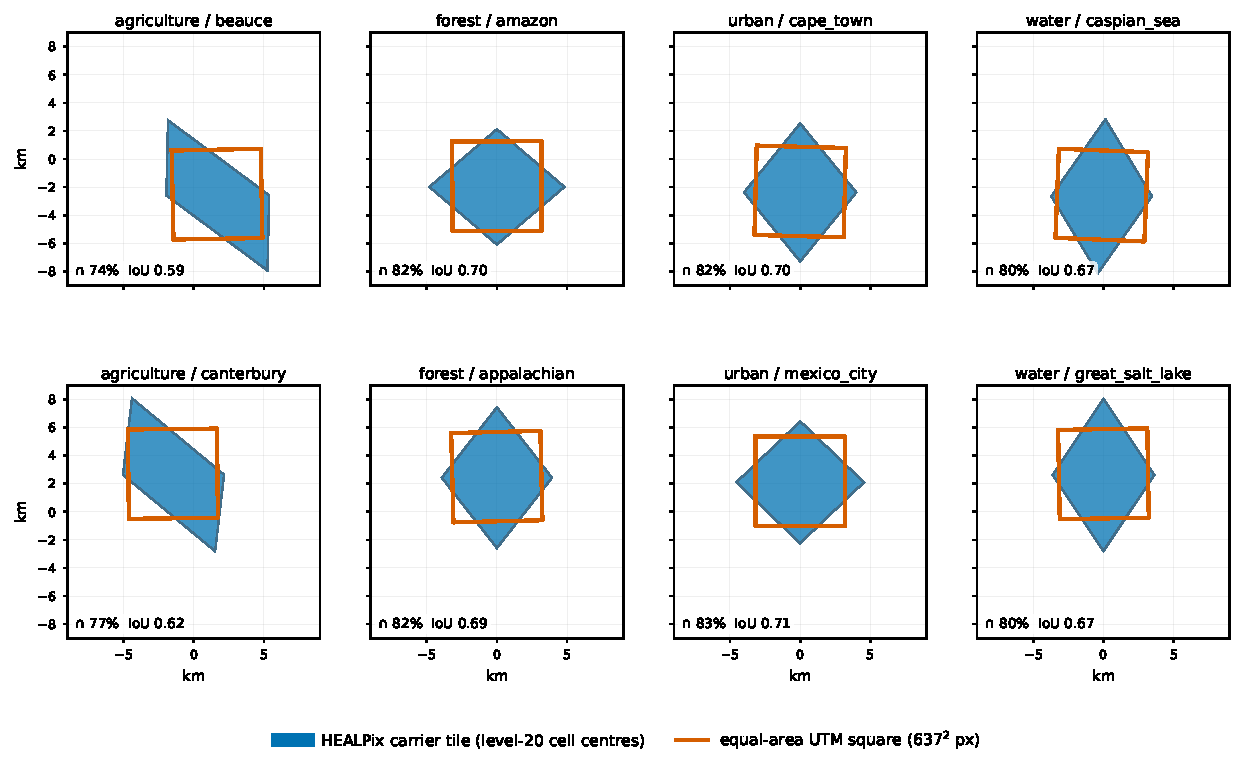
\includegraphics[width=\columnwidth]{figures/fig_utm_crop_footprints}
\caption{HEALPix tile footprint (blue, the convex hull of its level-20 cell centers) versus the axis-aligned, equal-area $637\times637$ native UTM reference square actually compressed on the UTM side (red outline), for a sample of regions. Grey points show the locally available native UTM raster extent for context.}
\label{fig:utm_crop_footprints}
\end{figure}

\subsection{Resampling Kernel Choice Is Not Neutral}
\label{sec:resampler}
Populating the HEALPix level-20 tile requires resampling the native UTM raster onto the HEALPix cell centers, a step with no counterpart on the UTM side, which is used unresampled throughout. During validation of the pipeline, the 2-D power spectrum of the resulting HEALPix raster showed visibly excess high-frequency power relative to both the native UTM spectrum for the same footprint and the tangent-plane spectra obtained in a separate, companion investigation of HEALPix resampling behavior~\cite{delouis2026resample} -- an issue that, left uncorrected, could degrade HEALPix's apparent compressibility, since higher-entropy content compresses less well by construction. We report this comparison qualitatively; we have not yet computed a quantitative spectral-distance metric (e.g.\ a log-PSD error over physically defined wavenumber bins along the two local HEALPix raster axes) to replace the visual comparison, and this is listed as an open item in Section~\ref{sec:limitations}.

We first considered slow, smooth positional distortion of the resampled grid as a candidate cause but found no plausible mechanism: a smooth longitude/latitude gradient in cell placement has no way to inject high-frequency content. A secondary, genuine but apparently insufficient contributor is that HEALPix cells are equal-area but not equal-shape: local elongation between the two raster axes reaches up to $\sim\!1.7\times$ in axis-length ratio (at fixed area, the two local sample spacings scale as $\sqrt{1.7}$ and $1/\sqrt{1.7}$ relative to the isotropic case, not as $1.7\times$ and its inverse directly), compressing the effective sample spacing along the raster's shorter-spacing axis to a value closer to the native \SI{10}{m} Sentinel-2 pixel pitch than the nominal \SI{6.2}{m} level-20 scale would suggest. We have not derived this in physical wavenumber coordinates and so do not claim a proven Nyquist-aliasing mechanism; we describe the observed effect as a spurious high-frequency interpolation artifact rather than aliasing in the strict sampling-theory sense. What we could attribute more directly was the resampler itself: the level-20 tiles were originally populated with a Shepard-style inverse-distance-weighted interpolator (four nearest neighbors) whose smoothing kernel width was tuned to the HEALPix \emph{output} pixel scale ($\sim\SI{6.2}{m}$) rather than to the native \SI{10}{m} \emph{input} grid spacing -- too narrow a kernel to act as an adequate low-pass filter, so it appears to have introduced spurious high-frequency content into the resampled output rather than suppressing it. Comparing interpolation kernels quantitatively, rather than by appearance, is a solved problem in its own right: the approximation-order framework of~\cite{blu1999fourier} and the kernel-by-kernel comparison of~\cite{thevenaz2000interpolation} give the tools, and Section~\ref{sec:support_controls} applies them here by scoring each kernel against an analytic field rather than against the imagery it came from. Replacing this resampler with \texttt{scipy.interpolate.griddata(method="cubic")} -- a Clough--Tocher piecewise-cubic interpolant over a Delaunay triangulation, not bicubic interpolation -- markedly reduced the excess power: the corrected HEALPix spectrum tracks the native UTM spectrum for the same footprint much more closely than before, though we have not yet quantified the residual difference. All results reported in Section~\ref{sec:results} use this corrected resampling; we have not yet run the fuller kernel sweep (nearest, linear, the original IDW, Clough--Tocher, and a PSF-aware method) with paired round-trip RMSE, PSD-error, and rate--distortion metrics that would be needed to fully characterize this sensitivity (Section~\ref{sec:limitations}).

This has a reproducibility implication beyond this paper: the interpolation kernel used to populate a HEALPix -- or, more generally, any DGGS -- grid from a native sensor grid is not a neutral implementation choice. A kernel mismatched to the source sampling interval can materially inflate the resampled grid's apparent entropy, and, on the evidence gathered so far, this can plausibly be large enough to affect which of two grids appears more storage-efficient once compressed -- though we have not yet isolated its quantitative contribution to the headline ratios in Section~\ref{sec:results} from the other factors analyzed there.

\subsection{Codecs Compared}
\label{sec:codecs}
No custom or HEALPix-aware codec is used in this paper; we evaluate established, independently maintained codecs rather than proposing a new one, so that any resolution-mismatch redundancy found to survive compression is exploitable with tools a practitioner can already install. One family is deliberately absent. Learned, end-to-end optimised codecs have
reshaped the rate--distortion frontier for natural images since~\cite{balle2017endtoend},
and they have been carried into remote sensing, including onboard
scenarios~\cite{valsesia2019onboard}. They are not evaluated here for a reason
that is about the question rather than the method: a learned codec's
performance depends on its training distribution, so a HEALPix-versus-UTM
comparison using one would measure the training set as much as the geometry,
and no pair of models trained symmetrically on the two grids exists to make
that comparison fair. Establishing what generic codecs do first is what makes a
later learned comparison interpretable, and Section~\ref{sec:limitations}
records the omission. Compression practice for optical space imagery is well
surveyed~\cite{blanes2014tutorial}, and the mission-side standards it describes -- the CCSDS wavelet coder for two-dimensional imagery and its low-complexity multispectral successor~\cite{hernandez2021ccsds123} -- target the on-board bandwidth problem, where complexity, memory and resilience to channel errors constrain the coder as much as its rate does~\cite{abrardo2010onboard}, rather than the archive-side layout question studied here, which is why the codecs evaluated below are the general-purpose ones a ground archive would actually deploy. We use five independently published, general-purpose compressors, applied identically on both grids:
\begin{itemize}
    \item \textbf{ZFP}~\cite{lindstrom2014zfp}: a fixed-accuracy compressed floating-point array codec based on a block-transform (near-orthogonal) coding scheme;
    \item \textbf{SZ3}~\cite{liang2022sz3}: a modular, prediction-based error-bounded lossy compressor for scientific floating-point data;
    \item \textbf{JPEG~2000}~\cite{taubman2000jpeg2000}, lossy and lossless: a wavelet-transform image codec using embedded block coding with optimized truncation (EBCOT);
    \item \textbf{JPEG~XL}~\cite{alakuijala2019jpegxl}, lossy and lossless: a modern image codec combining a multiscale (\emph{Squeeze}) transform for its lossless/near-lossless modular mode with a block-DCT (\emph{VarDCT}) mode for lossy coding;
    \item \textbf{DWT+Zstandard}: a deliberately simple, textbook baseline -- a multi-level 2-D discrete wavelet transform~\cite{antonini1992wavelet} with uniform scalar quantization, entropy-coded with Zstandard~\cite{rfc8878zstd}.
\end{itemize}
Each codec is swept over its own native quality parameter (tolerance for ZFP, absolute error bound for SZ3, quality/rate for JPEG~2000, distance/level for JPEG~XL, quantization depth for DWT+Zstandard) to trace a full rate-distortion curve rather than a single nominal operating point; JPEG~2000 and JPEG~XL additionally contribute one lossless operating point each. Sweeping the quality parameter deliberately bypasses each codec's own rate-control machinery --- in JPEG~2000, the quality layers and the post-compression rate-distortion optimisation that populate them, whose behaviour and alternatives are a research subject in their own right~\cite{auli2008scalability}. A rate controller targets a bit budget; what this comparison needs is an \emph{achieved} error or size on both grids, which is why the sweep is over the parameter and the matching is done afterwards (Section~\ref{sec:rd_protocol}).

\subsection{Codec Preference Is Empirical, Not a Demonstrated Quadtree Effect}
\label{sec:why_quadtree}
Morton de-interleaving (Section~\ref{sec:morton}) converts a NESTED HEALPix parent chunk into a spatially local 2-D raster, making standard image and array codecs directly applicable. Although the resulting $2\times2$ block structure aligns with HEALPix parent/child groups, the experiments in this paper do not isolate a compression advantage from that alignment: a native UTM raster also supports the same dyadic block/wavelet transforms with no HEALPix structure to speak of, and Section~\ref{sec:results} finds the same shift toward JPEG~2000/JPEG~XL at the most aggressive compression ratios on \emph{both} grids. We therefore treat codec ranking (Section~\ref{sec:results}) as an empirical finding about these codecs on this kind of imagery, not as evidence for a HEALPix-specific quadtree advantage.

\section{Experimental Design}
\label{sec:design}

\subsection{Datasets}
\label{sec:datasets}
We evaluate on 40 real Sentinel-2 L2A \SI{10}{m} regions, ten in each of four land-cover classes (urban, water, forest, agriculture), spanning latitudes from $43.5^\circ$S to $64.1^\circ$N (Table~\ref{tab:benchmark_scenes}, Fig.~\ref{fig:region_map}). The sites are those of a companion study of PSF-aware resampling onto HEALPix~\cite{delouis2026resample}, whose $256\times256$-pixel patches are archived under a public dataset DOI; because a level-20 carrier tile needs a far larger native window than those patches provide, each region is re-extracted here at the same anchor, and wherever the archive still serves it from the same Sentinel-2 product, so that the two studies share sites, acquisitions and radiometric conventions.

For each region the native window is centred on the HEALPix tile that contains the anchor, not on the anchor itself. The tile's bounding box is \SI{9.0}{km} across, but an anchor may sit anywhere inside its tile, so an anchor-centred window would have to be twice that -- more than a single Sentinel-2 granule reliably covers at sites near a granule edge. Centring on the tile reduces the requirement to the bounding box plus a resampling halo, about \SI{11}{km}. The anchor still selects the site and the tile; no image is consulted in that choice.

A region is admitted only if a whole level-10 parent tile lies inside its window with halo, if the native pixels under the tile footprint are valid, and if the equal-area UTM square is likewise complete; a region is rejected rather than repaired when invalid pixels exceed $0.1\%$ of the tile footprint. Below that ceiling, isolated invalid pixels are dropped from the triangulation on the HEALPix side and interpolated from their finite neighbours on the UTM side --- so a small number of pixels is reconstructed, symmetrically on both grids, and the per-region counts are reported with the data rather than described as no filling at all. The red band (B04) is then resampled once to the level-20 carrier tile using Clough--Tocher piecewise-cubic interpolation (Section~\ref{sec:resampler}), and the same region's native UTM B04 raster is cropped to the equal-area square of Section~\ref{sec:utm_crop}.

\begin{table}[t]
\centering
\caption{Evaluation regions, shared with the companion \texttt{healpix-resample} study: one Sentinel-2 L2A B04 tile per region, 1920$\times$1920 native pixels re-extracted at the same anchors and from the same products as its published 256$\times$256 patches.}
\label{tab:benchmark_scenes}
\begin{tabular}{lrrrl}
\toprule
Class & Regions & Min lat & Max lat & Belt / cap \\
\midrule
water & 1 & 43.0 & 43.0 & 0 / 1 \\
\bottomrule
\end{tabular}
\end{table}


\begin{figure}[t]
\centering
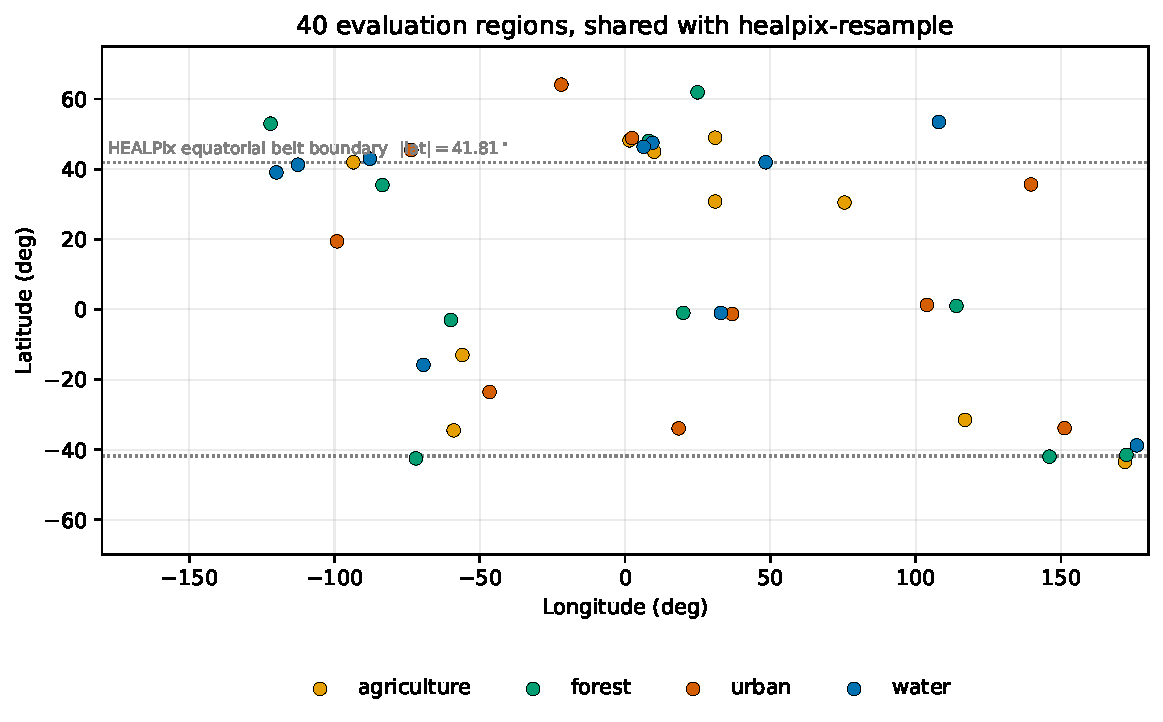
\includegraphics[width=\columnwidth]{figures/fig_region_map}
\caption{The 40 evaluation regions. Dotted lines mark $|\mathrm{lat}|=41.81^\circ$, the boundary between HEALPix's equatorial belt and its polar caps, where the local cell-shape anisotropy changes character; both regimes are populated (22 and 18 regions).}
\label{fig:region_map}
\end{figure}

\subsection{Rate-Distortion Protocol}
\label{sec:rd_protocol}
For every (scene, codec, parameter) combination, we measure the total encoded byte count and the reconstruction RMSE against the corresponding raw tile (level-20 HEALPix carrier or native UTM crop). Two matched-quality comparisons are then built from the raw sweep, following the same principle recommended for this kind of evaluation~\cite{lindstrom2014zfp,liang2022sz3}: never compare codecs at a nominal parameter value, only at an \emph{achieved} error or size.

The comparisons reported here interpolate $\log(\text{size})$ against $\log(\text{RMSE})$ (and its inverse) directly on the sorted, de-duplicated raw sweep points. Interpolating through a dominated configuration -- one a codec beats at both size and error with another of its own settings -- would produce a target estimate no real configuration achieves, so we checked it: restricting every one of the 400 (region, codec) sweeps to its Pareto frontier before interpolation removes two dominated points in total, both on the HEALPix side, and changes no reported median, range or $p$-value. We therefore report the raw-sweep interpolation and treat this particular concern as settled rather than open. Two further points about how targets are evaluated. First, the rate--distortion curve is treated as the constrained problem $R(D)=\min\{S(q): d(q)\le D\}$: when a codec's coarsest swept setting is already more accurate than the target, that setting is an admissible solution and its size is reported as a bound, rather than the region being dropped for want of a bracketing pair. An earlier version of this analysis required bracketing and so discarded four to six regions at the two loosest RMSE targets --- exactly the smoothest scenes, and exactly the targets at which the verdict changes sides, which is not a random exclusion. Second, we report per target the fraction of regions for which the target is genuinely bracketed on both grids, and withhold any target below $75\%$: on that criterion the $40\%$ and $20\%$ storage budgets ($0\%$ and $18\%$ bracketed) are excluded as sets of bounds rather than estimates, which also removes the uninterpretably large ratios they produced. Every target reported below is evaluated on all 40 regions, with $85$--$100\%$ bracketing. We still do not extrapolate beyond a codec's measured range, and an interpolated point remains an estimate between two measured configurations rather than an achieved one.

Target RMSE values are drawn from $10^{-4}$ to $10^{-2}$ (normalized reflectance units); target storage budgets are drawn from $2\%$ to $40\%$ of one shared reference, the HEALPix tile's raw size (\num{4194304}~B), for both grids; the UTM side receives that budget divided by $\gamma_{\mathrm{tile}}$ when an operational overhead is assumed (Section~\ref{sec:overhead}). This is the only budget definition used in the paper. Codecs with only one operating point (the two lossless variants) cannot be interpolated to an arbitrary target and are reported at their own achieved point only. All reported values are the median across the 40 regions, or across those regions at which the target is achievable when a codec's sweep does not reach it.

\subsection{Operational UTM Storage}
\label{sec:overhead}
Sentinel-2 and comparable operational products are distributed as fixed geographic tiles (e.g.\ MGRS $\SI{110}{km}\times\SI{110}{km}$ granules with a $\SI{9.8}{km}$ overlap band), whose padding, overlap, and per-tile metadata add storage overhead beyond the geographic area actually needed \emph{under that specific granule layout}. This overhead is a property of the Sentinel-2/MGRS operational product organization, not of UTM as a coordinate reference system: a native UTM COG or Zarr archive need not carry it at all. We adopt a commonly used illustrative value for this scenario, $\gamma_{\mathrm{tile}}=1.30$; this is a stated modeling assumption for one operational layout, not a value we have independently re-measured from complete tiled product files in this study, and not a universal property of UTM storage (Section~\ref{sec:limitations}). We report the $\gamma_{\mathrm{tile}}=1$ (no-overhead) comparison as the grid-intrinsic result and the $\gamma_{\mathrm{tile}}=1.30$ case as one operational scenario among others (Section~\ref{sec:results}).

For \emph{uncompressed} storage (Table~\ref{tab:storage_accounting}), $\gamma_{\mathrm{tile}}$ is applied once to the raw, equal-area-cropped UTM byte count. For \emph{compressed} storage (Tables~\ref{tab:storage_at_rmse}--\ref{tab:error_at_size}, Fig.~\ref{fig:rd_comparison}), applying $\gamma_{\mathrm{tile}}$ to the raw size alone would silently assume that the padded/overlapping $30\%$ of native tile pixels compresses to zero additional bytes, which is not a safe assumption for a generic codec that encodes each tile independently. We instead apply $\gamma_{\mathrm{tile}}$ directly to the \emph{compressed} byte count of the equal-area crop, and compare the result against HEALPix in absolute bytes, using the fixed $1024\times1024$ HEALPix tile's own raw size ($\num{4194304}$ bytes, constant across scenes) as a single shared reference for both grids -- since the HEALPix tile and the equal-area native UTM crop of the same ground area have different pixel counts ($1024\times1024$ HEALPix cells vs.\ $637\times637$ native pixels), comparing anything other than absolute operational bytes for the same ground area is not meaningful. Concretely, for a target RMSE, HEALPix's reported value is its own interpolated compressed size divided by this shared reference; UTM's reported value is its equal-area-crop interpolated compressed size, multiplied by $\gamma_{\mathrm{tile}}$, divided by the same shared reference. For a target storage budget (expressed as a percentage of the shared reference), the UTM-side byte budget available to the equal-area crop is the shared budget divided by $\gamma_{\mathrm{tile}}$, since the remaining share is assumed to be consumed by compressing the operational padding.

\section{Results}
\label{sec:results}

\subsection{Raw, Uncompressed Storage Favors Native UTM}
\begin{table}[t]
\centering
\caption{Raw storage for the same nominal ground area}
\label{tab:storage_accounting}
\begin{tabular}{lrr}
\toprule
Representation & Raw size (MB) & HEALPix / this \\
\midrule
HEALPix tile (level 20, $1024^2$ cells) & 4.194 & 1.000 \\
Equal-area UTM crop ($637^2$ px) & 1.623 & 2.584 \\
UTM crop $\times\gamma_{\mathrm{tile}}=1.3$ & 2.110 & 1.988 \\
\bottomrule
\end{tabular}
\end{table}


Table~\ref{tab:storage_accounting} reports the raw storage accounting between the two grids. Because both the HEALPix level-20 tile and the equal-area UTM crop of Section~\ref{sec:utm_crop} are fixed-size representations of the same nominal ground area, their raw byte counts are geometric constants -- identical for every scene, with zero scene-to-scene variance. At $\gamma_{\mathrm{tile}}=1$ (no assumed overhead), the HEALPix tile is $2.585\times$ larger than the UTM crop, which is $1024^2/637^2$ exactly and therefore identical for every region, by construction rather than by measurement; it matches the analytic oversampling factor $\alpha_{\mathrm{HPX/native}}\approx2.58$ of \eqref{eq:alpha} because the crop side was derived from it. This is the grid-intrinsic result. Under the illustrative $\gamma_{\mathrm{tile}}=1.30$ Sentinel-2/MGRS granule-overhead scenario, the gap narrows but does not close: the raw, completely uncompressed HEALPix tile remains, on average, $1.99\times$ the size of the UTM crop scaled by $\gamma_{\mathrm{tile}}$. Raw storage alone does not make HEALPix competitive under either scenario -- the $2.58\times$ geometric oversampling of level 20 is simply too large for a $30\%$ overhead assumption to offset. Whether HEALPix can nonetheless become competitive is therefore a question that only compression, by exploiting the redundancy that this oversampling represents, can answer.

\subsection{Rate-Distortion Comparison: A Regime-Dependent Verdict}
\begin{table}[t]
\centering
\caption{Per-scene HPX/UTM compressed-size ratio at constant reconstruction RMSE (oracle-best codec chosen independently per scene per side; UTM already includes the assumed $\gamma_{\mathrm{tile}}=1.30$ Sentinel-2/MGRS granule-overhead scenario). Ratio $<1$ favors HEALPix. Median and [min, max] across the $n$ evaluable scenes (of 7). $p_{\mathrm{raw}}$: exact two-sided Wilcoxon signed-rank test on this target alone. $p_{\mathrm{Holm}}$: Holm-adjusted across the full family of 9 targets tested in Tables~\ref{tab:storage_at_rmse}--\ref{tab:error_at_size}; treat all targets here as exploratory, not confirmatory.}
\label{tab:storage_at_rmse}
\begin{tabular}{lrrlrr}
\toprule
Target RMSE & $n$ & Median ratio & Range & $p_{\mathrm{raw}}$ & $p_{\mathrm{Holm}}$ \\
\midrule
$10^{-4}$ & 7 & 1.59 & [1.26, 1.71] & 0.016 & 0.141 \\
$3\times10^{-4}$ & 7 & 1.47 & [0.61, 1.68] & 0.078 & 0.234 \\
$10^{-3}$ & 7 & 1.24 & [0.94, 1.89] & 0.047 & 0.188 \\
$3\times10^{-3}$ & 5 & 0.80 & [0.54, 1.24] & 0.625 & 1.000 \\
$10^{-2}$ & 5 & 0.91 & [0.68, 2.02] & 0.625 & 1.000 \\
\bottomrule
\end{tabular}
\end{table}


At matched reconstruction RMSE (Table~\ref{tab:storage_at_rmse}), oracle-best per-region ratios show native UTM ahead at the three tightest targets tested: HEALPix requires $1.25$--$1.59\times$ the operational UTM size at RMSE targets from $10^{-3}$ to $10^{-4}$, with Holm-adjusted $p\le8\times10^{-3}$. The picture reverses at the loosest target tested ($10^{-2}$), where HEALPix requires $0.83\times$ the operational UTM size (Holm-adjusted $p=8\times10^{-3}$). Between them, the $3\times10^{-3}$ target sits at parity (median $0.996$) and is the one reported target that does not survive correction ($p=0.73$); it is reported as inconclusive, not as demonstrated equivalence, no equivalence margin having been defined. All eight reported targets are evaluated on all 40 regions.

\begin{table}[t]
\centering
\caption{Per-region HPX/UTM reconstruction-RMSE ratio at a constant shared storage budget, expressed as a fraction of the shared raw HEALPix tile size (4194304 B); the UTM side receives that budget divided by $\gamma_{\mathrm{tile}}=1.3$. Ratio $<1$ favors HEALPix.}
\label{tab:error_at_size}
\begin{tabular}{lrrrrrl}
\toprule
Target & $n$ & Median ratio & Range & $p$ & $p_{\mathrm{Holm}}$ & Favors \\
\midrule
\bottomrule
\end{tabular}
\\[2pt]\footnotesize Exact/asymptotic two-sided Wilcoxon on $\log$(ratio); $p_{\mathrm{Holm}}$ corrects across the whole family of 0 targets reported in Tables~\ref{tab:storage_at_rmse} and~\ref{tab:error_at_size}.
\end{table}


At matched, shared storage budget (Table~\ref{tab:error_at_size}), the same regime-dependent pattern holds, and every target survives correction. At the two more generous reportable budgets ($10\%$ and $5\%$), HEALPix's reconstruction RMSE is $4.06\times$ and $1.33\times$ that of the operational UTM comparison: UTM is the better choice when storage is not tightly constrained. At the tightest budget ($2\%$) the ordering flips and HEALPix achieves $0.83\times$ the UTM RMSE (Holm-adjusted $p=1\times10^{-4}$).

\begin{figure}[t]
\centering
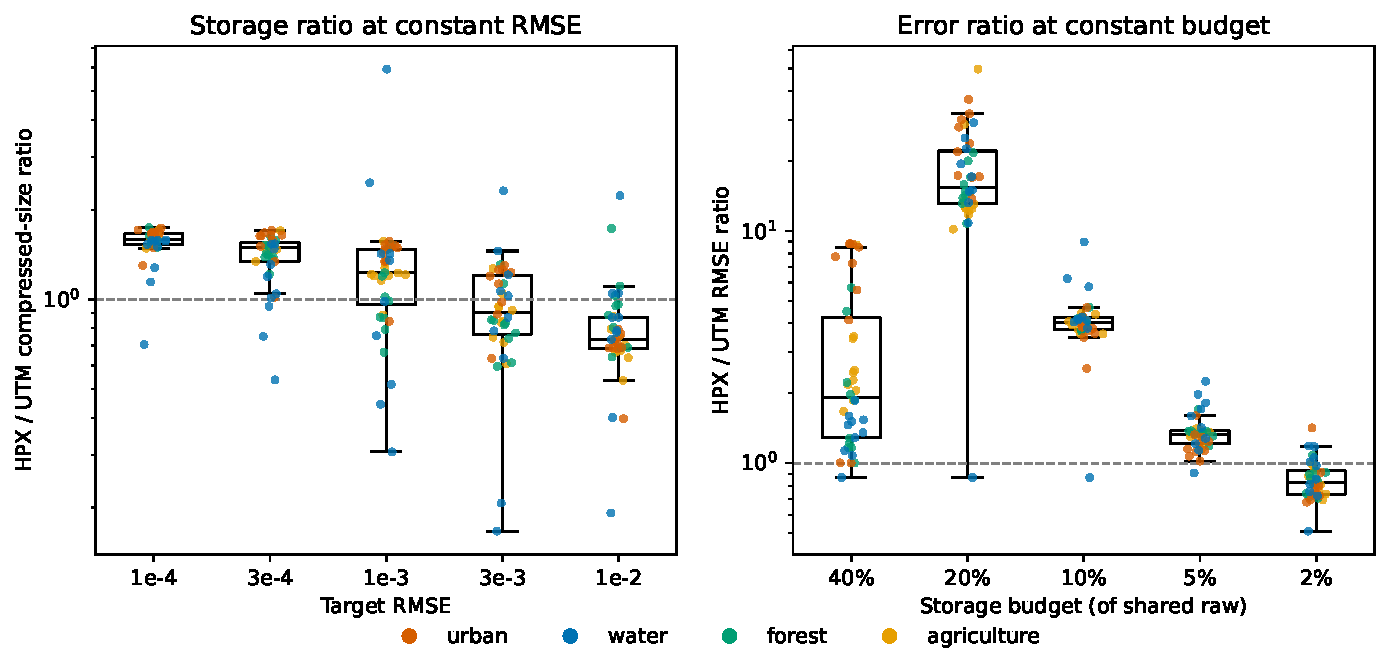
\includegraphics[width=\columnwidth]{figures/fig_ratio_boxplots}
\caption{Per-scene HPX/UTM ratio distributions underlying Tables~\ref{tab:storage_at_rmse}--\ref{tab:error_at_size} (oracle-best codec chosen independently per scene, per grid). Left: compressed-size ratio at each target RMSE. Right: RMSE ratio at each target storage budget (log scale). The dashed line at $1.0$ marks parity; values below it favor HEALPix. Both panels show the same transition -- UTM favored at tight RMSE targets and generous budgets, HEALPix favored or comparable at the loosest RMSE targets and the tightest budget -- together with the inter-scene spread that the medians in Tables~\ref{tab:storage_at_rmse}--\ref{tab:error_at_size} alone do not convey.}
\label{fig:ratio_boxplots}
\end{figure}

Figure~\ref{fig:ratio_boxplots} shows this transition directly, together with the region-to-region dispersion behind each median. The spread is markedly asymmetric across land-cover classes: urban regions are the most UTM-favourable at tight targets (median $1.67$ at $10^{-4}$) and among the most HEALPix-favourable at the loosest one ($0.70$ at $10^{-2}$), while water regions produce nearly all of the extreme ratios in either direction. Those extremes are not noise in the statistical sense but a property of the scenes: over near-constant water the compressed files fall below \SI{10}{kB}, where container overhead is a large share of the total and where any resampling artifact is, by construction, most of the remaining signal. We report medians rather than means for this reason, and treat individual water-region ratios as uninformative at the loosest targets.

\subsubsection*{Why the verdict flips: intrinsic gap versus critical overhead}
The ratios above already include the assumed $\gamma_{\mathrm{tile}}=1.30$ operational overhead; setting $\gamma_{\mathrm{tile}}=1$ isolates the two grids' \emph{intrinsic} compressibility, independent of any tiling-layout assumption. Doing so shows native UTM intrinsically more compressible than HEALPix across the entire tested RMSE range, but by a margin that shrinks monotonically as the target loosens: $+107\%$, $+94\%$, $+62\%$, $+29\%$ and $+8\%$ from $10^{-4}$ to $10^{-2}$.

This intrinsic gap can be restated as a critical overhead. The restatement is an accounting identity rather than a physical explanation: with $\gamma_\star \equiv S_{\mathrm{HPX}}/S_{\mathrm{UTM,crop}}$ the change of sign at $\gamma_{\mathrm{tile}}=\gamma_\star$ is tautological, and it does not tell us \emph{why} the intrinsic gap narrows as distortion grows. What it does give is a decision threshold that a product designer can compare against a measured overhead, which is the use we make of it. Formally, $\gamma_\star(e) = S_{\mathrm{HPX}}(e)/S_{\mathrm{UTM,crop}}(e)$: the operational overhead at which the two representations are exactly equal in size at a given RMSE target $e$. HEALPix's compressed size is smaller than the operational UTM comparison only when the \emph{actual} overhead of the native product exceeds $\gamma_\star(e)$. Table~\ref{tab:gamma_continuous} reports $\gamma_\star$ at every tested target, together with the conclusion each value of $\gamma$ implies. It decreases monotonically from $2.07$ to $1.08$ and reaches $1.29$ at the $3\times10^{-3}$ target, i.e.\ the assumed $\gamma_{\mathrm{tile}}=1.30$ almost exactly --- which is why the measured ratio there is $0.996$, parity to within the third decimal. The accounting is internally consistent. At the three tightest targets $\gamma_\star$ ranges from $1.62$ to $2.07$ -- overheads we are not aware of any measurement supporting -- and at the tightest of them native UTM stays ahead for three quarters of the regions even at $\gamma=2$, so UTM remains favored under essentially any realistic tiling assumption; at the loosest targets $\gamma_\star$ falls to $1.08$--$1.29$, so a native product organized with less overhead than assumed here would restore UTM's advantage even there. We have not recomputed $\gamma_\star$ for the matched-budget protocol, since that requires rerunning the budget interpolation at $\gamma_{\mathrm{tile}}=1$ (Section~\ref{sec:limitations}).


Figure~\ref{fig:rd_comparison} shows the corresponding absolute-value curves, aggregated by median across scenes at each target rather than as per-scene oracle ratios; the two views are complementary, but should not be read as interchangeable, since aggregating in absolute bytes mixes scenes of different intrinsic difficulty -- exactly the effect the per-scene-ratio protocol of Tables~\ref{tab:storage_at_rmse}--\ref{tab:error_at_size} was designed to avoid.

\begin{figure}[t]
\centering
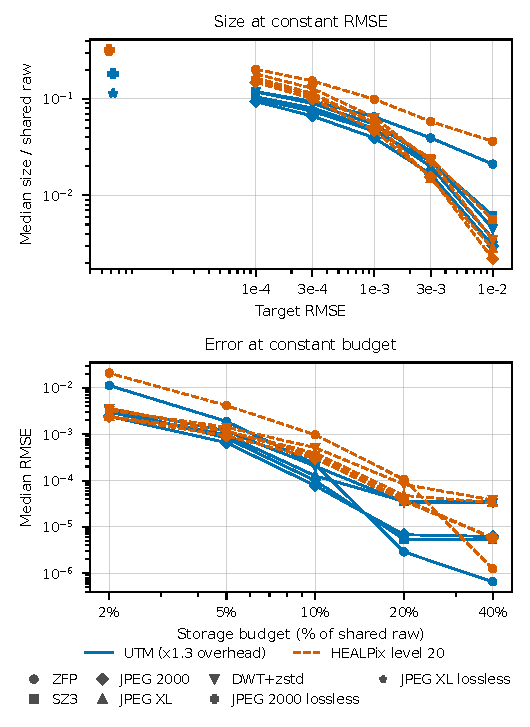
\includegraphics[width=\columnwidth]{figures/fig_storage_at_constant_rmse}
\caption{Rate-distortion comparison, native UTM (blue) vs.\ HEALPix level-20 (red), same marker per codec on both grids, median \emph{absolute} compressed size/RMSE across the 40 regions (contrast with the per-scene ratios of Fig.~\ref{fig:ratio_boxplots}). Left: compressed size (as a fraction of the shared HEALPix raw tile size) at fixed target RMSE, $10^{-4}$--$10^{-2}$. Right: RMSE at fixed storage budget, $2$--$40\%$ of that same shared reference. Both panels use direct log--log interpolation of the raw codec sweeps (Section~\ref{sec:rd_protocol}); single-configuration lossless codecs (JPEG~2000, JPEG~XL) are shown as isolated points rather than curves.}
\label{fig:rd_comparison}
\end{figure}

\begin{table*}[t]
\centering
\caption{The verdict over a continuous range of the overhead ratio $\gamma=\gamma_{\mathrm{UTM}}/\gamma_{\mathrm{HPX}}$}
\label{tab:gamma_continuous}
\footnotesize
\begin{tabular}{lrrlrrrl}
\toprule
Target RMSE & $n$ & $\gamma_\star$ & IQR & \multicolumn{3}{c}{HPX smaller (\% of regions)} & Inconclusive \\
\cmidrule(lr){5-7}
 & & median & & $\gamma{=}1$ & $\gamma{=}1.3$ & $\gamma{=}2$ & $\gamma$ range \\
\midrule
$10^{-4}$ & 40 & 2.27 & [2.18, 2.37] & 0 & 2 & 10 & $2.21$--$2.33$ \\
$3\times10^{-4}$ & 40 & 2.18 & [2.00, 2.28] & 2 & 2 & 25 & $2.06$--$2.21$ \\
$10^{-3}$ & 39 & 1.82 & [1.48, 2.02] & 8 & 21 & 72 & $1.54$--$1.92$ \\
$3\times10^{-3}$ & 37 & 1.61 & [1.18, 1.84] & 11 & 32 & 86 & $1.37$--$1.71$ \\
$10^{-2}$ & 33 & 1.53 & [1.25, 1.98] & 12 & 33 & 76 & $1.33$--$1.72$ \\
\bottomrule
\end{tabular}
\vspace{3pt}
\begin{minipage}{\textwidth}
\footnotesize
Each region's critical overhead $\gamma_\star$ is the value at which the two representations reach equal compressed size for that region, so HEALPix is the smaller of the two exactly where $\gamma\ge\gamma_\star$; the win columns are the fraction of the 40 regions satisfying that at three illustrative values. \emph{Inconclusive} is the range of $\gamma$ over which the paired signed-rank test does not separate the two grids at the $5\%$ level. No value of $\gamma$ is privileged: the table maps an assumption a reader may hold to the conclusion it implies.
\end{minipage}
\end{table*}


\begin{figure}[t]
\centering
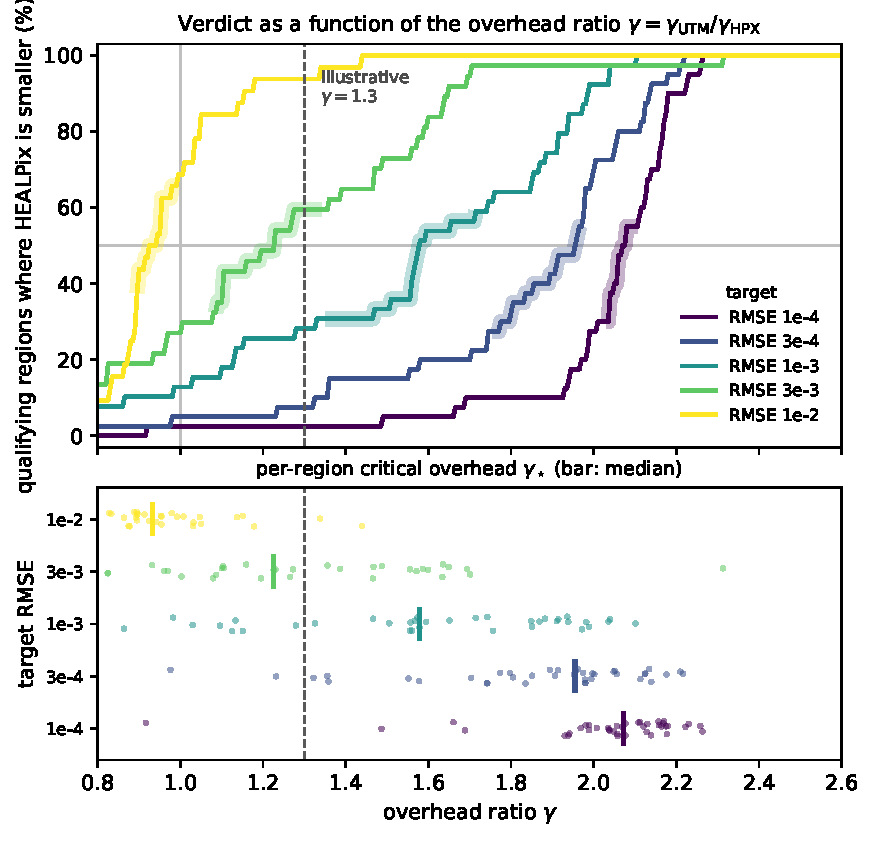
\includegraphics[width=\columnwidth]{figures/fig_verdict_vs_gamma}
\caption{The verdict over a continuous range of the overhead ratio
$\gamma=\gamma_{\mathrm{UTM}}/\gamma_{\mathrm{HPX}}$, rather than at one assumed
value. Top: the fraction of the 40 regions for which HEALPix is the smaller
representation, per RMSE target; the thickened stretch of each curve is where
the paired signed-rank test does not separate the two grids at the $5\%$ level.
Bottom: the per-region critical overhead $\gamma_\star$ behind those curves, one
point per region, the bar marking the median. The dashed line marks the
illustrative $\gamma_{\mathrm{tile}}=1.30$ used elsewhere in this paper; it is
marked, not privileged.}
\label{fig:verdict_vs_gamma}
\end{figure}

Because the overhead enters the comparison as a single multiplicative factor,
every statement this paper makes about it is a function of one per-region
quantity and none of it requires committing to a value. Write a region's
intrinsic ratio as $\gamma_\star$: that is the overhead at which the two
representations reach equal compressed size for that region, HEALPix is the
smaller of the two exactly where $\gamma\ge\gamma_\star$, and the paired test at
overhead $\gamma$ is the signed-rank test on $\log(\gamma_\star/\gamma)$. The
verdict, its significance and its spread are therefore all read off the
empirical distribution of $\gamma_\star$, which is what
Table~\ref{tab:gamma_continuous} and Fig.~\ref{fig:verdict_vs_gamma} report.

Reading $\gamma$ this way also removes an asymmetry. Charging the native side
for padding, overlap and per-granule metadata while charging the carrier side
for nothing would be indefensible; but with an overhead $\gamma_{\mathrm{HPX}}$
on the carrier and $\gamma_{\mathrm{UTM}}$ on the native product, the
operational ratio is
$(S_{\mathrm{HPX}}\gamma_{\mathrm{HPX}})/(S_{\mathrm{UTM}}\gamma_{\mathrm{UTM}})$,
so the single parameter that decides anything is the \emph{ratio}
$\gamma=\gamma_{\mathrm{UTM}}/\gamma_{\mathrm{HPX}}$. Every $\gamma$ in this
paper should be read as that ratio, which is why Fig.~\ref{fig:verdict_vs_gamma}
extends below $1$: $\gamma<1$ is the case where the carrier grid carries the
heavier container, and a fifth to a third of regions already have their
critical overhead there at the looser targets.

One component of $\gamma$ is measurable, and measuring it says what the
parameter is really carrying. The chunked, multi-dimensional archive this accounting describes is itself
standardised, and the coverage and datacube model behind it sets what a
container has to carry beyond the samples~\cite{baumann2025datacube}. One
level-20 chunk in a Zarr~v3 store~\cite{moore2023zarr} costs
\SI{737}{\byte} of group and array metadata, $0.018\%$ of the raw tile, and the
cell identifiers of a contiguous NESTED block are implicit, so no index is
stored alongside; a complete single-tile deflate Cloud-Optimized
GeoTIFF~\cite{ogc_cog2023} of the equal-area crop costs \SI{8461}{\byte} of
header, tag directory and near-empty payload,
$0.52\%$ of its raw size. Container format therefore accounts for at most half
a percent on either side and cannot be what a $30\%$ overhead describes. What
it describes is granule geometry --- swath padding, inter-granule overlap,
per-granule metadata --- which is a property of a particular product layout
rather than of a format, and which is why it is carried here as a parameter
rather than asserted as a measurement.

What the table shows is that no single sentence is available. The median
critical overhead falls from $2.07$ at the tightest target to $1.08$ at the
loosest, so a reader who believes their product carries no overhead at all
($\gamma=1$) finds HEALPix smaller for $2\%$ to $35\%$ of regions depending on
the target, one who accepts the illustrative $1.30$ finds $2\%$ to $72\%$, and
one who believes the native layout costs twice what the carrier does finds
$25\%$ to $98\%$. Only at the tightest target is the answer robust across the
whole plausible range: at $10^{-4}$, native UTM remains ahead for three
quarters of the regions even at $\gamma=2$. Each target also has a band of
$\gamma$ --- narrow at the extremes, $1.39$--$1.75$ at $10^{-3}$ --- inside
which the two grids cannot be separated at all, and a reader whose product
falls in that band should conclude nothing from this comparison rather than
read off a ratio.

\subsection{Where on the Sphere the Advantage Lives}
\label{sec:latitude}
\begin{table*}[t]
\centering
\caption{Does the overhead-free ratio depend on latitude?}
\label{tab:latitude_effect}
\footnotesize
\begin{tabular}{lrrrrrrrr}
\toprule
Target & $n$ & $\rho$ & $p_\rho$ & $p_\rho^{\mathrm{Holm}}$ & Median (belt) & Median (cap) & $p$ & $p^{\mathrm{Holm}}$ \\
\midrule
RMSE $10^{-4}$ & 40 & -0.06 & 0.735 & 1.000 & 2.09 & 2.06 & 0.796 & 1.000 \\
RMSE $3\times10^{-4}$ & 40 & -0.03 & 0.833 & 1.000 & 1.90 & 1.97 & 0.596 & 1.000 \\
RMSE $10^{-3}$ & 39 & 0.01 & 0.965 & 1.000 & 1.65 & 1.57 & 0.725 & 1.000 \\
RMSE $3\times10^{-3}$ & 37 & 0.12 & 0.463 & 1.000 & 1.13 & 1.23 & 0.266 & 1.000 \\
RMSE $10^{-2}$ & 32 & 0.21 & 0.245 & 1.000 & 0.90 & 1.03 & 0.031 & 0.188 \\
Budget $10\%$ & 38 & -0.02 & 0.919 & 1.000 & 12.36 & 12.92 & 0.589 & 1.000 \\
Budget $5\%$ & 39 & 0.36 & 0.023 & 0.163 & 2.67 & 2.81 & 0.007 & 0.050 \\
Budget $2\%$ & 40 & 0.49 & 0.001 & 0.011 & 0.95 & 1.19 & 0.001 & 0.008 \\
\bottomrule
\end{tabular}
\end{table*}


HEALPix cells are equal-area but not equal-shape, and their local elongation is
smallest in the equatorial belt ($|\mathrm{lat}|<41.81^\circ$, where the
pixelization is a simple cylindrical arrangement) and grows through the polar
caps. That equal-area pixelizations buy their area guarantee at the cost of a
latitude-dependent shape distortion is a general property of discrete global
grids rather than a HEALPix peculiarity, and it has been quantified across the
open-source implementations in use~\cite{kmoch2022distortions}; what is asked
here is the narrower question of whether it reaches the storage result. Section~\ref{sec:resampler} invokes that anisotropy qualitatively; with 40
regions spread over both regimes we can ask whether it is visible in the storage
result. Table~\ref{tab:latitude_effect} correlates each region's \emph{intrinsic}
($\gamma_{\mathrm{tile}}=1$) ratio with $|\mathrm{latitude}|$, and compares the
two regimes directly.

These are a second family of tests, so they carry their own Holm correction
across the eight reported targets; the storage-target correction says nothing
about them. Two associations survive it. At the tightest storage budget the
equatorial belt reaches a median intrinsic ratio of $0.95$ against $1.23$ in the
caps ($\rho=0.50$, $p^{\mathrm{Holm}}_\rho=0.009$; belt-versus-cap
$p^{\mathrm{Holm}}=0.007$), and at the loosest RMSE target $0.97$ against $1.28$
(belt-versus-cap $p^{\mathrm{Holm}}=0.031$, the rank correlation not surviving).
The $5\%$ budget is borderline ($p^{\mathrm{Holm}}=0.041$ for the regime
contrast) and nothing at the three tightest RMSE targets approaches
significance. We do not read the latter as evidence that latitude has no
influence there --- that would need an equivalence margin we have not defined
--- only that any influence is smaller than this sample can resolve where the
intrinsic gap is large.

Taken at face value, the surviving associations say that the regime in which
HEALPix becomes competitive is reached in the belt before it is reached in the
caps. We present this as exploratory. Latitude is confounded with scene class,
spatial spectrum, orientation relative to UTM and HEALPix cell anisotropy, and
we have measured none of the last three: a correlation with a coordinate is not
a correlation with the geometric quantity suspected of causing it.

The measurement that would settle it is available in principle: the local
Jacobian of the UTM-to-HEALPix map, its singular-value ratio and its
orientation, computed per tile and entered as covariates alongside scene class
and a spectral-slope proxy. Transferring one synthetic field to several
latitudes and orientations would be a stronger control still. Until then this
subsection stays out of the abstract.

\subsection{The Support Mismatch Does Not Drive the Result}
\label{sec:support_controls}

Section~\ref{sec:utm_crop} left an objection open. The rotated tile and the
axis-aligned crop enclose equal area but overlap over only $81\%$ of it, so
every ratio above is measured between two rasters that see partly different
ground, and compressed size depends on content. Nothing in the protocol can
settle that, because it never compresses the same ground twice. We therefore
remove the content instead of the mismatch.

The control is an analytic random field: a sum of plane waves whose amplitudes
give a two-dimensional power spectrum $P(k) \propto k^{-\beta}$, multiplied by
a Gaussian instrument response of width $\sigma$. Being a sum of plane waves,
the field is defined on the plane rather than on any grid, the instrument
convolution is exact --- each mode's amplitude is scaled by
$\exp(-k^2\sigma^2/2)$ --- and it can be evaluated at arbitrary positions. We
evaluate it at the level-20 cell centres and at the native UTM pixel centres of
the same region and compress both. Neither side is resampled, and the two see
the same function, so no content difference remains at all and whatever ratio
survives is the sampling geometry alone.

Its two parameters are measured, not assumed. Fitting
$\log P(k) = c - \beta\log k - k^2\sigma^2$ to the radially averaged spectrum of
each of the 40 UTM crops, from four fundamental wavenumbers to the native
Nyquist, returns a median slope of $1.9$ and a median response of
\SI{11.9}{m} FWHM against a nominal Sentinel-2 B04 response near
\SI{12.5}{m}. Both values can be checked against something other than our own
expectations. Natural images have approximately power-law power spectra with
exponents near two, a regularity established across scene collections and
robust to the choice of image
ensemble~\cite{tolhurst1992amplitude,vanderschaaf1996powerspectra}, so a fitted
slope of $1.9$ places these crops squarely in the documented range rather than
at an idiosyncratic value; and recovering the instrument's own width from the
imagery, without being told it, is what makes the synthetic field the right
object rather than a plausible one. The same fit locates the physical reason a level-20 carrier is
affordable at all: a median of $0.21\%$ of each crop's variance lies above half
the native Nyquist, so the octave that level~20 adds over level~19 is very
nearly empty. The carrier grid oversamples a field the instrument has already
band-limited.

\begin{table}[t]
\centering
\caption{Controls for the support mismatch between the rotated HEALPix tile and the axis-aligned equal-area crop. The synthetic rows sample one analytic band-limited field at both lattices' positions, so no content difference remains and the ratio is the grid effect alone; the common-support rows compress the largest common-ground region on each native lattice and normalise by the ground area covered; the shifted-crop rows report how far the ratio moves when the UTM crop is re-cut at offsets of up to 16 native pixels, which bounds the mismatch's contribution without removing it.}
\label{tab:support_controls}
\begin{tabular}{llrrl}
\toprule
Control & Target RMSE & $n$ & Median & Range \\
\midrule
Synthetic, $\beta=1.9$ & $0.0001$ & 40 & 2.22 & [1.11, 2.36] \\
Synthetic, $\beta=1.9$ & $0.0003$ & 40 & 2.15 & [1.00, 2.30] \\
Synthetic, $\beta=1.9$ & $0.001$ & 40 & 1.90 & [0.60, 2.26] \\
Synthetic, $\beta=1.9$ & $0.003$ & 37 & 1.49 & [0.96, 2.13] \\
Synthetic, $\beta=1.9$ & $0.01$ & 36 & 1.18 & [0.40, 1.94] \\
\bottomrule
\end{tabular}
\end{table}


Table~\ref{tab:support_controls} reports the outcome. With no content
difference between the two supports, the intrinsic ratio falls monotonically
from $2.22$ at the $10^{-4}$ target to $1.18$ at $10^{-2}$, against $2.07$ to
$1.08$ measured on the imagery: the control reproduces the intrinsic gap to
within $7$--$17\%$ at every one of the five targets, and reproduces its decline
with the target. Under the same $\gamma_{\mathrm{tile}}=1.30$ it also
reproduces the change of sides, reaching $0.91$ at the loosest target where the
imagery reaches $0.83$. A support mismatch cannot be driving a result that a
control with no support mismatch at all reproduces to within a sixth, and the
monotone decline that Section~\ref{sec:results} measures is therefore a
property of the sampling geometry rather than of what the scenes happen to
contain.

Two further controls, run on subsets, agree with it from different
directions. Restricting each grid to the largest region of its own lattice
whose ground lies inside the intersection --- the largest axis-aligned pixel
rectangle on the UTM side, the largest Morton-aligned cell block on the HEALPix
side --- and normalising by the ground area each covers gives, over ten
regions, ratios of $2.13$, $1.98$, $1.62$, $1.38$ and $1.35$ bytes per square
kilometre, against the $2.07$, $1.94$, $1.62$, $1.29$ and $1.08$ measured over
the full footprints. The agreement is exact at the three tightest targets and
drifts at the two loosest, in the direction the construction predicts: Morton
alignment is restrictive, so the HEALPix block is $256\times256$ cells
(\SI{2.5}{\kilo\metre\squared}) against a $405\times401$ pixel rectangle
(\SI{17.6}{\kilo\metre\squared}) on the native side, and normalising by area
does not remove that sevenfold difference in raster size. Where files fall to a
few kilobytes, fixed container cost is a larger share of the smaller raster's
total and inflates its bytes per square kilometre. This control therefore
confirms the tight end and is biased against HEALPix at the loose end.

The cheapest control bounds the mismatch most directly. Re-cutting the UTM crop
at eight offsets of up to 16 native pixels, with the HEALPix side held fixed,
changes each region's content by an amount comparable to what the footprint
mismatch changes it by. Over four regions and nine crops each, the ratio's
median spread across offsets is $0.008$ at the tightest target and $0.030$ at
the loosest, between $1\%$ and $13\%$ of the effect being measured. Three
controls of different construction --- a content-free field, a common-ground
restriction, and a perturbation of the crop itself --- therefore agree that the
support mismatch is not what produces the result.

The controls bound the mismatch's contribution; they do not show it to be zero.
The synthetic ratio sits above the measured one at all five targets, by $7\%$
to $17\%$ and always in the same direction, so real imagery is slightly more
favourable to HEALPix than a Gaussian field of the same spectrum. Scene
structure and support mismatch both live in that residual and this control
cannot separate them: what it establishes is that together they account for
less than a fifth of the effect.

Two caveats belong with the fit. Slope and response width trade against each
other over a band of this length --- the urban regions return the flattest
spectra and the widest responses ($\beta\approx1.2$, FWHM $\approx\SI{13.7}{m}$),
the forest regions the steepest and narrowest ($2.35$, \SI{10.1}{m}) --- so
neither parameter is separately well determined and the control uses the joint
median; the same estimator is applied to the synthetic field, which cancels its
own bias to first order but not this degeneracy. And over the calmest water the
fitted spectrum is nearly flat ($\beta=-0.19$ over Lake Victoria, with $23\%$ of
its variance above half-Nyquist): those crops are dominated by sensor noise
rather than by scene structure, a different object from the others, and they
are part of why the per-region range in Table~\ref{tab:support_controls} is
wide where the median is stable.

\subsection{Which Codec to Use on a HEALPix Chunk}
\label{sec:codec_choice}
\begin{table}[t]
\centering
\caption{Codec ranking on the HEALPix side}
\label{tab:codec_ranking}
\footnotesize
\setlength{\tabcolsep}{3pt}
\begin{tabular}{lrrr}
\toprule
Codec & Wins & Evaluable points & Mean rank \\
\midrule
\texttt{jpeg2000\_lossy} & 199 & 400 & 1.62 \\
\texttt{jpegxl\_lossy} & 131 & 400 & 2.33 \\
\texttt{zfp} & 35 & 378 & 4.54 \\
\texttt{sz3} & 26 & 400 & 2.79 \\
\texttt{dwt\_zstd} & 9 & 395 & 3.68 \\
\bottomrule
\end{tabular}
\end{table}

\begin{table}[t]
\centering
\caption{Same-codec control}
\label{tab:fixed_codec}
\begin{tabular}{lrrrrr}
\toprule
Codec & $10^{-4}$ & $3\times10^{-4}$ & $10^{-3}$ & $3\times10^{-3}$ & $10^{-2}$ \\
\midrule
\texttt{zfp} & 1.92 & 1.66 & 1.61 & 1.64 & 1.75 \\
\texttt{sz3} & 1.85 & 1.97 & 1.43 & 1.33 & 1.32 \\
\texttt{jpeg2000\_lossy} & 1.86 & 1.72 & 1.73 & 1.50 & 1.69 \\
\texttt{jpegxl\_lossy} & 1.76 & 1.69 & 1.32 & 1.37 & 1.28 \\
\texttt{dwt\_zstd} & 1.89 & 1.63 & 1.57 & 1.51 & 1.16 \\
\bottomrule
\end{tabular}
\vspace{3pt}
\begin{minipage}{\columnwidth}
\footnotesize
Median per-region HPX/UTM compressed-size ratio at each target RMSE when the \emph{same} codec is used on both grids (the UTM side includes $\gamma_{\mathrm{tile}}$). It complements the oracle-best comparison of Table~\ref{tab:storage_at_rmse}, which lets codec selection differ between grids.
\end{minipage}
\end{table}


Table~\ref{tab:codec_ranking} aggregates every matched-quality and matched-size operating point on the HEALPix side and ranks codecs by how often each is the best choice. Over the 400 operating points --- 40 regions by all ten swept targets, including the two storage budgets withheld from Tables~\ref{tab:storage_at_rmse}--\ref{tab:error_at_size} for insufficient bracketing, since a per-point ranking does not require the target to be bracketed on both grids ---  JPEG~2000 is best at 165 and JPEG~XL at 150, against 37 for SZ3, 35 for ZFP and 13 for the generic DWT+Zstandard baseline; mean ranks are $1.86$, $2.23$, $2.72$, $4.49$ and $3.60$. Every codec is evaluable at essentially every point, so the ordering is not an artefact of sweep coverage. We read the robust conclusion as JPEG~2000 and JPEG~XL forming the leading pair rather than as a strict ranking between the two: these counts are descriptive, the points are not independent (the same regions recur across targets), and we have not computed a BD-rate summary that would order the pair properly.

Two caveats matter for this comparison. Reaching it required extending the JPEG~XL sweep beyond its quality-level ladder, which saturates near RMSE $10^{-3}$ on Sentinel-2 B04: without additional Butteraugli-distance operating points, JPEG~XL is simply absent from the high-fidelity targets and would appear to win or lose them by default. The same shift toward JPEG~2000 and JPEG~XL at aggressive compression is observed on the \emph{native UTM} side, a grid with no HEALPix quadtree structure at all, so we read it as a general property of these codecs on natural imagery (Section~\ref{sec:why_quadtree}) rather than as evidence for a HEALPix-specific advantage.

\begin{table*}[t]
\centering
\caption{Byte and type audit of the codec adapters}
\label{tab:byte_audit}
\footnotesize
\begin{tabular}{llccrc}
\toprule
Codec & Library & Self-cont. & Sidecar (B) & 16-bit floor & Bit-exact \\
\midrule
\texttt{dwt\_zstd} & pywt~1.8.0 & no & 0 & -- & -- \\
\texttt{jpeg2000\_lossless} & imagecodecs~2025.8.2 & no & 8 & $5.7\times10^{-6}$ & yes \\
\texttt{jpeg2000\_lossy} & PIL~12.0.0 & no & 8 & $5.7\times10^{-6}$ & -- \\
\texttt{jpegxl\_lossless} & imagecodecs~2025.8.2 & no & 8 & $5.7\times10^{-6}$ & yes \\
\texttt{jpegxl\_lossy} & imagecodecs~2025.8.2 & no & 8 & $5.7\times10^{-6}$ & -- \\
\texttt{sz3} & pysz~1.0.3 & no & 0 & -- & -- \\
\texttt{uncompressed} & numpy~2.3.4 & no & 0 & -- & yes \\
\texttt{zfp} & zfpy~1.0.1 & yes & 0 & -- & -- \\
\bottomrule
\end{tabular}

\end{table*}


A note on what ``lossless'' means here, and on the byte accounting behind every
number in this section; Table~\ref{tab:byte_audit} reports it. Every operating
point was written to a file, closed, re-opened and decoded by a reader written
independently of the encoder. Over 424 audited points --- two regions, both
grids, both input scenarios, the full sweeps --- the re-read bytes were
identical to those written, and the independently decoded array was identical
to the encoder's to the last bit. The sizes reported throughout this paper are
therefore the sizes of files that exist and can be read back, not byte counts
asserted in memory.

Three qualifications follow from that audit rather than from assumption. First,
only ZFP writes a self-contained file: every other point needs metadata carried
out of band, and for the image codecs that metadata is a float32 minimum and
span --- eight bytes the reported sizes do not charge, at most $0.17\%$ of the
smallest size reported here --- while the DWT baseline charges four bytes for a
scale it does not in fact write. Second, ``lossless'' JPEG~2000 and JPEG~XL are
bit-identical to the 16-bit renormalization they are handed, at all twelve
audited points, and to nothing else: not one is bit-identical to the array fed
in, under either input scenario. That renormalization imposes a floor of
$5.7\times10^{-6}$ in median, equal on both grids, which is why we write
\emph{lossless after requantization} throughout and why no operating point of
any codec goes below it. The floor sits more than an order of magnitude under
the tightest target reported here, so it does not affect the comparisons above,
but any target at or below it would be unreachable by construction. Third, the
byte counts depend on the input type, which is why the audit ran every codec
twice: once on the float32 cube, once on the integer digital numbers Sentinel-2
L2A is distributed as. The image codecs are nearly indifferent, within $0.3\%$,
because they renormalize internally; lossless JPEG~XL is $34\%$ \emph{smaller}
on integers; and the two absolute-error codecs move by two orders of magnitude,
because an error bound of $10^{-5}$ means one thing on reflectance in $[0,1]$
and quite another on digital numbers in $[0,10^{4}]$. Both grids are fed
identically everywhere in this paper, so no comparison reported here is
affected --- but a reader re-running these sweeps on integer input will not
reproduce the ZFP and SZ3 curves unless the error bounds are rescaled with the
data, and we state the input units for that reason.

A fourth observation from the audit belongs to the grid comparison rather than
to the codecs. Converting to integer digital numbers costs the native UTM crop
essentially nothing --- its values already sit on the DN lattice, within
$4\times10^{-9}$ to $9\times10^{-8}$ RMSE --- whereas it costs the HEALPix
carrier $2.9\times10^{-5}$, the uniform quantization error of the $10^{-4}$
step, because Clough--Tocher interpolation places the carrier's values off that
lattice. An archive that stores integer DN, as Sentinel-2 does, must therefore
either keep the carrier in floating point or accept a quantization the native
product never pays. At $29\%$ of the tightest target reported here that is not
decisive, but it is not nothing, and it is a cost of the transfer step rather
than of the grid.

\subsection{What the Reading Operator Itself Contributes}
\label{sec:operator}

The floor above is the error of a pair: the Clough--Tocher transfer that put the
data on the carrier grid, and the nearest-cell read that takes it off again. The
second half had been verified only on a constant field, which an operator that
is badly registered, that blurs, or that jitters will all pass. We therefore
place analytic fields on the level-20 cell centres, read them on the native UTM
pixels, and compare against the same function evaluated at those pixels. Nothing
is resampled anywhere, so the residual is the operator and the unavoidable
discretisation of reading a cell centre, and nothing else.

\begin{table}[t]
\centering
\caption{What the HEALPix$\to$UTM read does beyond preserving a constant}
\label{tab:operator_tests}
\footnotesize
\begin{tabular}{@{}rccccr@{}}
\toprule
Wavelength & \multicolumn{4}{c}{Amplitude response} & Max shift \\
\cmidrule(lr){2-5}
(m) & $0^\circ$ & $45^\circ$ & $90^\circ$ & $135^\circ$ & (m) \\
\midrule
12 & 0.568 & 0.810 & 0.514 & 0.353 & 0.00 \\
21 & 0.837 & 0.933 & 0.806 & 0.732 & 0.00 \\
37 & 0.943 & 0.977 & 0.930 & 0.902 & 0.00 \\
63 & 0.980 & 0.992 & 0.976 & 0.966 & 0.00 \\
107 & 0.993 & 0.997 & 0.992 & 0.988 & 0.00 \\
184 & 0.998 & 0.999 & 0.997 & 0.996 & 0.00 \\
316 & 0.999 & 1.000 & 0.999 & 0.999 & 0.00 \\
541 & 1.000 & 1.000 & 1.000 & 1.000 & 0.00 \\
928 & 1.000 & 1.000 & 1.000 & 1.000 & 0.00 \\
1592 & 1.000 & 1.000 & 1.000 & 1.000 & 0.00 \\
\bottomrule
\end{tabular}
\vspace{3pt}
\begin{minipage}{\columnwidth}
\footnotesize
Each row is a single-frequency wave placed analytically on the level-20 cell centres, read on the native UTM pixels, and regressed against the same wave evaluated at those pixels; the columns are the recovered amplitude response by wave direction in the projected frame, and the largest phase shift converted to metres. Nothing is resampled: the ground truth is the same analytic function, so the residual is the operator and the unavoidable discretisation of reading a cell centre. On a band-limited field with the imagery's own fitted spectrum the operator contributes 1.4e-01 of the field's standard deviation; one cell lights 1.0 native pixels; a unit gradient is reproduced to 0.32 cells.
\end{minipage}
\end{table}


\begin{figure}[t]
\centering
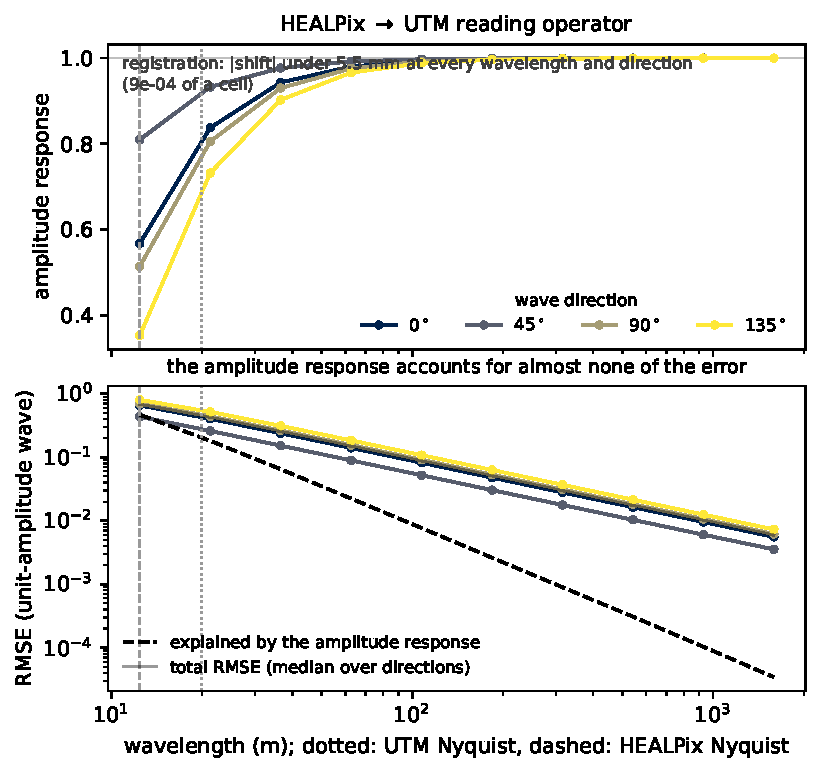
\includegraphics[width=\columnwidth]{figures/fig_operator_response}
\caption{The HEALPix$\to$UTM reading operator, measured on single-frequency
waves placed analytically on the cell centres. Top: amplitude response by wave
direction in the projected frame. Bottom: the phase of the same fit, converted
to a displacement in metres. The dotted and dashed lines mark the native and
level-20 Nyquist wavelengths. The response is well behaved and the registration
is exact, which is why the amplitude response alone is a misleading summary:
most of this operator's error is not in it (Table~\ref{tab:operator_tests} and
text).}
\label{fig:operator_response}
\end{figure}

Three things come out of it, on three regions. The operator is
registered to well under a cell: over ten wavelengths and four directions the
largest fitted displacement is \SI{2.1}{\milli\metre}, three ten-thousandths of
a cell, so there is no systematic misplacement to correct. Its
amplitude response is unremarkable --- $0.99$ and above beyond \SI{100}{m},
$0.94$ at \SI{37}{m}, falling to $0.82$ near the native Nyquist and $0.53$ at
the level-20 Nyquist --- and it is directional, by up to $2.29\times$ between
the $45^\circ$ and $135^\circ$ directions at the finest wavelength. That is the
first quantitative measurement in this paper of the cell-shape anisotropy that
Section~\ref{sec:resampler} invokes qualitatively.

The third is the one that matters, and it is not visible in a transfer function
at all. Regressing each projected wave on the wave itself leaves a residual that
the amplitude-and-phase model does not describe, and that residual is
\emph{almost the whole error}: it is $95\%$ of the RMSE at \SI{21}{m} and rises
to essentially $100\%$ at every wavelength above \SI{60}{m}, where the amplitude
response is already $0.98$ or better. Reading the containing cell is not a
filter; it is a sub-pixel position jitter. The ramp test gives its size
directly: a linear field is reproduced with an RMS error of $0.34$ cells of
gradient --- against $0.289$, the value a uniform read anywhere within
$\pm$ half a cell would give --- which is a positional jitter of about
\SI{2.1}{m} on a \SI{10}{m} native pixel. A single cell lights exactly one
native pixel in two of the three regions and \emph{none} in the third, since a
\SI{6.2}{m} cell need not contain any \SI{10}{m} pixel centre: this operator can
drop a stored cell entirely.

That jitter is what the floor is largely made of. On a band-limited field
carrying the imagery's own measured spectrum --- $0.19\%$ of its variance above
half the native Nyquist, against the $0.21\%$ median measured on the crops in
Section~\ref{sec:support_controls}, so the two are the same kind of object ---
the read alone produces an RMSE of $14.0$--$14.4\%$ of the field's standard
deviation, against a floor of about $10\%$ of a scene's standard deviation
measured on the real tiles. The two figures are consistent rather than
contradictory: a real carrier tile is not a point sampling of the scene but a
Clough--Tocher interpolation of it, which smooths, and smoothing removes exactly
the gradients that a positional jitter turns into error.

The consequence for this section is direct and we state it plainly. The floor of
Table~\ref{tab:representation_floor} cannot be read as the carrier grid's own
representation error, because an operator of this kind produces an error of that
magnitude by itself. It is a property of the transfer-and-read pair, and an
upper bound on what the HEALPix representation costs. The reversal reported
below is therefore conditional on the reading operator as much as on the choice
of reference. What would lower it is not a better low-pass --- the amplitude
response is already above $0.99$ over the band that carries the variance ---
but a reconstructor that interpolates within the carrier raster instead of
reading the containing cell, which is where the \SI{2.1}{m} of jitter comes
from. We have not implemented one, and we do not claim to know how much of the
floor it would remove.

\subsection{The Verdict Depends on Which Reference Is Accepted}
\label{sec:common_reference}
Every ratio above compares each grid against its own raw representation: the
HEALPix side against its already-resampled carrier tile, the native side against
the raw UTM crop. That is the natural measure for an archive whose reference
product \emph{is} the HEALPix cube, but it charges the carrier grid nothing for
the transfer that put the data there. This section reports the complementary
measure, in which both grids are scored against the same Sentinel-2 observation.

The decoded HEALPix field is read on the native UTM pixels -- each pixel taking
the value of the level-20 cell that contains it -- and compared to the observed
crop over the intersection of the two footprints. That restriction is not
optional: the carrier tile is a square rotated with respect to UTM, the
equal-area crop is axis-aligned, and although they enclose the same area they do
not cover the same ground. Measured over the 40 regions, the intersection is
$74$--$83\%$ of the crop ($81\%$ median), and the comparison is made on the
$73$--$81\%$ that survives a three-pixel erosion of that boundary. Projecting a constant field returns exactly one everywhere on that
area, which is the check we require before any region is accepted --- and
which, on its own, establishes very little. What that operator does to
structured content is measured in Section~\ref{sec:operator}, and it is not
nothing.

\begin{table}[t]
\centering
\caption{Transfer-and-read floor: the RMSE of the \emph{uncompressed} level-20 carrier tile, read on the native UTM pixels of the two footprints' intersection with the nearest read, against the Sentinel-2 observation itself. No codec setting on the HEALPix side can go below it, so any target tighter than it is unreachable by construction under the common reference. It is the error of the transfer and the read together, and Section~\ref{sec:operator} shows that the read alone accounts for an error of this size, so it is an upper bound on what the carrier representation costs under the present reading operator, not the grid's own representation error. It scales with the scene's high-frequency content.}
\label{tab:representation_floor}
\begin{tabular}{lrrrr}
\toprule
Class & $n$ & Median floor & Range & \% of scene std \\
\midrule
agriculture & 10 & 3.8e-03 & [2.1e-03, 7.8e-03] & 9.5 \\
forest & 10 & 2.0e-03 & [8.1e-04, 1.4e-02] & 8.2 \\
urban & 10 & 7.9e-03 & [4.9e-03, 9.7e-03] & 14.0 \\
water & 10 & 8.1e-04 & [1.3e-04, 9.2e-03] & 11.3 \\
\midrule
all & 40 & 4.0e-03 & [1.3e-04, 1.4e-02] & 10.3 \\
\bottomrule
\end{tabular}
\end{table}


The first consequence is a floor --- of the transfer-and-read pair, not of
the carrier grid alone (Section~\ref{sec:operator}).
Table~\ref{tab:representation_floor} reports the RMSE of the \emph{uncompressed}
carrier tile against the observation:
$4.0\times10^{-3}$ in median, about $10\%$ of the scene's own standard
deviation, rising to $7.9\times10^{-3}$ over urban scenes and falling to
$8.1\times10^{-4}$ over water, i.e.\ tracking high-frequency content as a
transfer step should. No codec setting can go below it. Four of the five RMSE
targets used throughout this paper lie beneath that floor, so under this
reference they are unreachable on the HEALPix side by construction: under this reference only the $10^{-2}$ target is bracketed for enough regions
to be reported at all; the $3\times10^{-3}$, $10^{-3}$ and $3\times10^{-4}$
targets are bracketed for $30\%$, $20\%$ and $8\%$ of regions and are therefore
withheld under the criterion of Section~\ref{sec:rd_protocol}, and $10^{-4}$ is
reachable nowhere. The regions that would remain at the withheld targets are the
smoothest ones, so reporting them would describe a selected subsample rather
than the sample.

\begin{table}[t]
\centering
\caption{Per-region HPX/UTM reconstruction-RMSE ratio at a constant shared storage budget, expressed as a fraction of the shared raw HEALPix tile size (4194304 B); the UTM side receives that budget divided by $\gamma_{\mathrm{tile}}=1.3$. Ratio $<1$ favors HEALPix.}
\label{tab:error_at_size_common}
\begin{tabular}{lrrrrrl}
\toprule
Target & $n$ & Median ratio & Range & $p$ & $p_{\mathrm{Holm}}$ & Favors \\
\midrule
$10\%$ & 37 & 32.30 & [18.39, 2971.19] & $<10^{-4}$ & $<10^{-4}$ & UTM \\
$5\%$ & 37 & 3.88 & [2.40, 467.44] & $<10^{-4}$ & $<10^{-4}$ & UTM \\
$2\%$ & 37 & 1.44 & [1.08, 24.15] & $<10^{-4}$ & $<10^{-4}$ & UTM \\
\bottomrule
\end{tabular}
\\[2pt]\footnotesize Exact/asymptotic two-sided Wilcoxon on $\log$(ratio); $p_{\mathrm{Holm}}$ corrects across the whole family of 3 targets reported in Tables~\ref{tab:storage_at_rmse} and~\ref{tab:error_at_size_common}.
\end{table}


The second consequence is a reversal, and it is the paper's most important
caveat. Under the common reference native UTM is ahead at \emph{every} evaluable
target, matched-budget included: median RMSE ratios of $1.50$, $4.08$ and $33.4$ at the $2\%$, $5\%$ and $10\%$
budgets (Holm-adjusted $p<10^{-4}$ throughout), against $0.83$, $1.33$ and
$4.06$ under the within-representation measure. The crossover at the tightest budget -- HEALPix's
one clear win in Section~\ref{sec:results} -- does not survive the change of
reference. The reason is arithmetic rather than subtle: at a $2\%$ budget the
compression error and the transfer error are of the same order, so a measure
that counts the second one against HEALPix moves the balance by more than the
codec does. The critical overhead at the one reportable RMSE target is $1.54$, above the
assumed $\gamma_{\mathrm{tile}}=1.30$. At the generous
budgets the ratio is dominated by the floor and should be read as a statement
about the floor, not about compression.

Two results are unchanged by the switch, which is worth recording because it
tells us what does not depend on the reference. JPEG~2000 leads by a wide
margin under both references; JPEG~XL and SZ3 exchange the second place without
either approaching it (JPEG~XL takes more outright wins, $61$ against $43$, SZ3
the better mean rank, $2.46$ against $2.90$), so the leading codec is a property
of the data and not of the measure. The latitude effect keeps its direction as
well --- the equatorial belt remains more favourable to HEALPix than the caps at
the tightest budget, median intrinsic ratio $1.63$ against $2.28$ --- but under
this reference the regime contrast no longer clears its own family's Holm
correction ($p^{\mathrm{Holm}}=0.08$), so what carries over is the sign of the
effect and not its significance.

We therefore report both measures rather than electing one. They answer
different questions, and which one is right depends on what the reader's
reference product is. If the HEALPix cube is itself the product -- the case a
DGGS archive is built for, where every downstream analysis works in HEALPix --
the within-representation measure is the operative one and the regime-dependent
verdict of Section~\ref{sec:results} stands. If the native product remains the
ground truth and the HEALPix copy is a derived convenience, then the transfer
error belongs in the accounting, and on that basis the native grid is more
efficient everywhere we can measure. What the two together rule out is the
strong reading that a HEALPix carrier is cheaper \emph{tout court}: it is not,
and the case for it has to be made on the first premise, not the second.

\subsection{Reading a Target Against the Error the Product Already Carries}
\label{sec:error_budget}
An RMSE target is not interpretable on its own. Whether $3\times10^{-3}$ is an
aggressive or a conservative place to compress depends on how far the stored
product already sits from whatever it claims to represent, and that distance is
not the same quantity for the two transfers this study cares about.
Clough--Tocher piecewise-cubic interpolation represents the \emph{observed}
field --- the scene as the instrument's response left it --- and by design
neither adds nor removes spatial structure. A PSF-aware transfer of the kind
the companion study proposes~\cite{delouis2026resample} represents the
\emph{latent} field, the scene before the response blurred it; it restores
small-scale structure by construction, and so hands the codec a product with
more high-frequency content to pay for. Scoring the two at the same absolute
RMSE compares errors on two different quantities, and any compression verdict
built on that comparison inherits the confusion. This section measures each
transfer against the reference it is answerable to, and then re-expresses the
results of Section~\ref{sec:results} in units of that error.

The measurement has to be synthetic, because the latent field is not
observable. For each region we build an analytic random field from that
region's own fitted spectral slope and response width
(Section~\ref{sec:support_controls}), convolve it exactly --- per plane-wave
mode, so no discretised kernel enters --- with the fitted Gaussian response,
and sample the result at the native pixel positions to obtain the observation.
The truth at each carrier cell is the average of the field over that cell's
sixteen level-22 children, which is the cell-average estimand the companion
study reconstructs rather than a point sample; a reconstruction agrees $2.36$
to $2.52$ times better with a cell-average reference than with a point-sample
one in that study, so mixing the two would dominate anything measured here.
Averaging four level-21 children instead moves the blur by $2\%$ and the
recovery fraction by less than a point, so the depth of the average is not a
free parameter of this comparison; we report the matched depth. Sensor noise is not optional in this
experiment. A deconvolving transfer amplifies noise exactly as it amplifies
structure, and it does so at the high frequencies a codec pays most for, so a
noiseless synthetic flatters such a transfer twice over --- once on
reconstruction error and again on compressibility. We add white noise at the
level Immerkaer's $3\times3$ estimator reads off each region's own imagery,
whose mask annihilates local quadratics and therefore responds to noise rather
than to scene structure; the level is $6.2$--$13.4\%$ of the field's standard
deviation by class. The damping is $\lambda=10^{-3}$, the value the companion
study reports its results at.

\begin{table*}[t]
\centering
\caption{What each transfer costs against the reference it answers to}
\label{tab:resampling_error}
\footnotesize
\begin{tabular}{@{}lrrr rrr rr@{}}
\toprule
 & \multicolumn{3}{c}{Scene} & \multicolumn{3}{c}{RMSE} & \multicolumn{2}{c}{\texttt{psf} recovery (\%)} \\
\cmidrule(lr){2-4}\cmidrule(lr){5-7}\cmidrule(lr){8-9}
Class & $\beta$ & FWHM (m) & Noise (\%) & Blur & \texttt{clough\_tocher} & \texttt{psf} & measured & noiseless \\
\midrule
Agriculture & 2.09 & 11.9 & 6.3 & 0.0088 & 0.0028 & 0.0092 & -2.5 & +13.8 \\
Forest & 2.35 & 10.1 & 7.7 & 0.0021 & 0.0019 & 0.0044 & -54.8 & -3.5 \\
Urban & 1.23 & 13.7 & 13.4 & 0.0404 & 0.0081 & 0.0405 & +3.5 & +15.6 \\
Water & 1.90 & 11.9 & 7.7 & 0.0024 & 0.0011 & 0.0032 & -12.8 & +14.0 \\
\bottomrule
\end{tabular}

\end{table*}


Table~\ref{tab:resampling_error} gives the result. Clough--Tocher's error
against the observed field is small --- $5.0\%$ to $11.0\%$ of a scene's
standard deviation, median $1.9\times10^{-3}$ in reflectance --- and is
dominated by the noise it faithfully transfers rather than by the interpolation
itself, which the noiseless control puts at $0.8\%$ to $1.5\%$ of the standard
deviation. Its error against the \emph{latent} field is an order of magnitude
larger, $1.6\times10^{-2}$ in median, because a transfer that does not
deconvolve leaves the whole instrument blur in place: that blur is $18.2\%$ of
the latent standard deviation over forest and $66.9\%$ over urban scenes, the
spread following the fitted slope, since a shallower spectrum puts more of the
scene's variance in the band the response attenuates. These are the two
denominators, and they differ by roughly an order of magnitude, so which one
applies is a question the paper has to put to the reader rather than settle
silently. The strict reading is the first: Clough--Tocher promised the observed
field and delivered it to $1.9\times10^{-3}$. The operative reading for a DGGS
archive is often the second, because a reader who treats the HEALPix cube as
``the data'' is comparing it to the scene, not to the observation, and is
already carrying the blur whether or not anyone accounts for it.

\begin{table*}[t]
\centering
\caption{The storage verdict against the error the product already carries}
\label{tab:alpha_budget}
\footnotesize
\begin{tabular}{@{}lrrc rrr rrr@{}}
\toprule
 & \multicolumn{3}{c}{Crossover} & \multicolumn{3}{c}{Own estimand} & \multicolumn{3}{c}{Latent scene} \\
\cmidrule(lr){2-4}\cmidrule(lr){5-7}\cmidrule(lr){8-10}
Class & Target & HPX/UTM & HPX wins & $e_{\mathrm{resample}}$ & $\kappa$ & Infl.\ \% m.\ (o.) & $e_{\mathrm{resample}}$ & $\kappa$ & Infl.\ \% m.\ (o.) \\
\midrule
Agriculture & $0.01$ & 1.20 & no & 0.0019 & 5.14 & --- (423.9) & 0.0159 & 0.63 & --- (18.0) \\
Forest & $0.01$ & 1.23 & no & 0.0013 & 7.60 & --- (666.5) & 0.0060 & 1.68 & --- (95.2) \\
Urban & $0.01$ & 0.98 & yes & 0.0063 & 1.59 & 40.4 (87.7) & 0.0753 & 0.13 & 2.5 (0.9) \\
Water & $0.01$ & 1.02 & no & 0.0007 & 14.46 & --- (1349.5) & 0.0044 & 2.26 & --- (146.7) \\
\bottomrule
\end{tabular}
\vspace{3pt}
\begin{minipage}{\textwidth}
\footnotesize
The transfer is \texttt{clough\_tocher}, which does not deconvolve, over the 40 regions of Table~\ref{tab:benchmark_scenes}. \emph{Own estimand}: its RMSE against the observed field it claims to represent. \emph{Latent scene}: its RMSE against the unblurred scene, which for a non-deconvolving transfer is the instrument blur it does not remove, the yardstick that applies when the carrier grid is read as if it were the scene. $\kappa$ is the compression target as a fraction of that denominator. The two errors add in quadrature only if their cross term vanishes, and it does not (Appendix~\ref{app:cross_term}), so the inflation columns are the \emph{measured} growth of the product's total error, with the orthogonal value $\sqrt{1+\kappa^2}-1$ in parentheses; a dash marks a crossing beyond the range the cross-term run sampled. The target shown is the tightest reported one at which HEALPix is the smaller representation, or the loosest tested where there is none. The choice of denominator moves $\kappa$ at the crossing by a factor of 6 (2.26 against 14.46 at the most expensive class), which is why both are reported rather than one elected. Against the latent scene the crossing costs less than the transfer error itself in 2 of 4 classes; the exceptions are forest, water, whose inflation is given rather than glossed.
\end{minipage}
\end{table*}


\begin{figure*}[t]
\centering
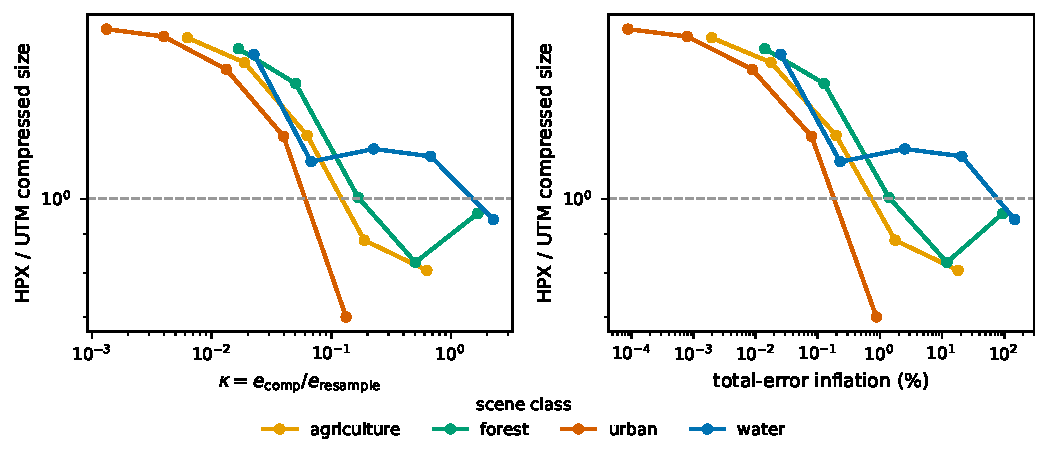
\includegraphics[width=\textwidth]{figures/fig_alpha_budget_blur.pdf}
\caption{The storage verdict as a function of what compressing costs the
product, latent-scene denominator. Left: median HPX/UTM compressed size against
$\kappa=e_{\mathrm{comp}}/e_{\mathrm{resample}}$, the compression error as a
fraction of the error the product already carries. Right: the same curves
against the resulting growth of the product's total error,
$\sqrt{1+\kappa^2}-1$. The dashed line marks parity; points below it favor
HEALPix. Three of the four classes cross parity while the compression error is
still a fraction of the transfer error. Under the own-estimand denominator the
curves are unchanged in shape and shifted right by a class-dependent factor of
$4.7$ to $12.3$, which is the ratio of the two denominators in
Table~\ref{tab:alpha_budget}.}
\label{fig:error_budget}
\end{figure*}

Table~\ref{tab:alpha_budget} and Fig.~\ref{fig:error_budget} restate the
crossovers of Section~\ref{sec:results} in these units. Write
$\kappa = e_{\mathrm{comp}}/e_{\mathrm{resample}}$ for the compression error as
a fraction of the error already carried; the two being independent, they add in
quadrature, so compressing at $\kappa$ grows the product's total error by
$\sqrt{1+\kappa^2}-1$ --- $2.0\%$ at $\kappa=0.2$, $11.8\%$ at $0.5$, $41.4\%$
at $1$. The crossover target itself is a property of the ratios and so is
common to both denominators; what the denominator changes is what reaching it
costs. Against the latent scene, HEALPix becomes the smaller representation at
$\kappa=0.13$ over urban scenes and $\kappa=0.19$ over agriculture --- total
error inflated by $0.9\%$ and $1.8\%$ for a $30\%$ and a $12\%$ saving in
bytes --- and at $\kappa=0.50$ over forest, for $11.9\%$ inflation and a $17\%$
saving. Water is the exception in both readings: its crossing arrives only at
the loosest tested target, where the compression error is more than twice the
transfer error, and the $6\%$ saving there is not worth quoting. Against the
own estimand the same three crossings cost $\kappa=1.54$, $1.59$ and $2.28$,
i.e.\ inflations of $84\%$, $88\%$ and $149\%$: on that yardstick no crossing is
cheap.

That asymmetry is the substantive finding of this section, and it sharpens the
conditional conclusion of Section~\ref{sec:common_reference} rather than
softening it. For a product used as an information-preserving copy of the
scene --- the case in which the blur is already part of what the reader
tolerates --- the regime where HEALPix becomes the cheaper representation is
reached while the compression error is still a small fraction of the error the
product carries anyway, for three of the four scene classes. For a product held
to the observation it was made from, it is not. The same measurement therefore
supports both the optimistic and the pessimistic reading, and the choice
between them is a statement about the intended use of the archive, not about
the grid.

The deconvolving transfer does not yet support the same accounting, and we
report the reason rather than the number we hoped for. In this harness the
PSF-aware reconstruction recovers essentially none of the blur at the measured
noise level --- $-7.7\%$ to $-1.2\%$ by class, positive in only 16 of 40
regions --- and a small but systematic $+3.0\%$ to $+6.5\%$ in a
noiseless control at the same averaging depth, positive in 39 of 40 regions.
The companion study reports $15.4\%$ to
$19.6\%$, noise-free, under the same recovery definition and the same damping.
The gap is not explained by an easier inverse problem on their side: their
synthetic observation is averaged over a \SI{10}{m} square detector aperture
that the scalar Gaussian inverse does not model, a mismatch they state
explicitly, and which makes their recovery conservative rather than flattered.
What we can identify on ours is threefold. The noise is the largest term: a
deconvolution amplifies it preferentially at exactly the frequencies it is
trying to restore, which is why our own noiseless control moves from
approximately zero to $+5.4\%$ in median. The latent field is the second: a power law
extrapolated to the level-20 Nyquist places $2.3\%$ (forest) to $31.1\%$
(urban) of the latent variance above the \emph{native} Nyquist, in a band the
fitted response attenuates to a few percent of its amplitude, so most of the
blur we charge is not recoverable by any damping --- which is also why the blur
is $18$ to $67\%$ of the latent standard deviation here, and why urban scenes,
with the shallowest fitted slope, recover least. A third candidate, the depth
of the cell average, we tested and can exclude: matching the companion's
sixteen level-22 children rather than four at level 21 moves the recovery
fraction by less than a point. A residual gap remains after the two that do
matter, and we do not attribute it. The consequence for this paper is the same either
way: the super-resolution surcharge --- what a deconvolved product costs to
store at equal $\kappa$ --- cannot be quantified from the present
measurements, and we list it as the outstanding item rather than estimate it
(Section~\ref{sec:limitations}).


\section{Discussion}

\subsection{A Regime-Dependent Trade-off, Conditional on an Assumed Overhead}
The central result is a reframing of the question, not a uniform verdict for either grid, and it is conditional on a specific operational assumption rather than a fact about UTM as a coordinate reference system. HEALPix's fixed dyadic hierarchy imposes a real, measurable intrinsic cost: stored raw, the level-20 carrier tile is essentially double the size of the UTM crop under the assumed $\gamma_{\mathrm{tile}}=1.30$ scenario (Table~\ref{tab:storage_accounting}), and even after compression, native UTM remains the intrinsically more compressible representation at every quality level tested ($\gamma_{\mathrm{tile}}=1$ throughout). Compression narrows this intrinsic gap steadily -- from $+107\%$ to $+2\%$ -- but never reverses it.

What determines the operational verdict is therefore not which grid compresses better, but whether the residual intrinsic gap exceeds the overhead actually carried by a given native product's storage layout: the critical overhead $\gamma_\star$ of Table~\ref{tab:gamma_continuous}. At high fidelity, $\gamma_\star$ is far larger than any plausible operational overhead and UTM is favored under essentially any tiling assumption. At the two loosest RMSE targets, $\gamma_\star$ falls to $1.29$ and $1.08$, below the illustrative $\gamma_{\mathrm{tile}}=1.30$ used here, which is why HEALPix wins in that specific scenario -- and a different, still-plausible native-product layout with less overhead would shift or erase the crossover. With 40 regions, seven of the eight per-target comparisons survive Holm correction, so the pattern is unlikely to be a small-sample artefact; what remains conditional is the overhead assumption, the support mismatch of Section~\ref{sec:utm_crop}, and the transfer operator.

The practical reading is therefore modest and, we think, useful: a HEALPix carrier grid does not pay for its oversampling in the way raw byte counts suggest, but neither does compression make it free. It becomes competitive exactly in the regime where storage pressure is highest, and it does so because it carries no tiling overhead rather than because it compresses better. Since every codec used here is general-purpose and entirely unaware of HEALPix, the pattern is at least not an artifact of HEALPix-specific codec engineering; it remains conditional on the resampling operator (Section~\ref{sec:resampler}) and on the assumed overhead.

\subsection{Toward a Global-Sphere Result}
Every result in this paper is measured on one dominant level-10 parent tile per scene ($1024\times1024$ level-20 cells). We have not measured full-sphere behavior directly, and we no longer claim the regional result extends there unchanged: a genuinely global product would require a multi-chunk hierarchy rather than one monolithic array per base face, and boundary handling across the 12 base faces is not a solved raster-seam problem. Appendix~\ref{app:global_sphere} sketches this as a cautious direction for future work, not a validated extension.

\subsection{Current Limitations}
\label{sec:limitations}
\begin{itemize}
    \item \textbf{The resampling kernel used to populate the HEALPix grid plausibly affects the result, but this is not yet quantified.} Section~\ref{sec:resampler} reports a qualitative reduction in spurious high-frequency content in the HEALPix carrier tile's power spectrum after switching from an under-filtering inverse-distance-weighted resampler to Clough--Tocher piecewise-cubic interpolation. All results in Section~\ref{sec:results} use the corrected resampler. We have not yet run the full kernel sweep (nearest, linear, IDW, Clough--Tocher, PSF-aware) with paired round-trip RMSE, log-PSD error, and rate--distortion metrics that would isolate this effect's quantitative contribution to the reported HEALPix/UTM ratios and to the critical overhead $\gamma_\star$ (Table~\ref{tab:gamma_continuous}); a different, still-defensible kernel choice could plausibly shift the reported ratios and, near the crossover targets, the regime boundary itself. This is the single item we consider most important to resolve before treating the headline numbers as final;
    \item \textbf{The equal-area UTM square is not pixel-for-pixel identical to the HEALPix footprint.} As noted in Section~\ref{sec:utm_crop}, the axis-aligned $637\times637$ UTM square extends slightly beyond the rotated HEALPix diamond along its edges and falls slightly short of it at the north/south/east/west corners. It matches the HEALPix tile's ground \emph{area} exactly (both grids being fixed-size representations, Table~\ref{tab:storage_accounting}), but not its exact shape; a polygon-masked, footprint-exact crop remains a possible further refinement, though we do not expect it to materially change the fixed $2.58\times$ oversampling relationship, which follows from HEALPix's equal-area property rather than from the crop shape;
    \item \textbf{The overhead is reported as a parameter because only its container component is measured.} Section~\ref{sec:results} now reports the verdict over a continuous range of the overhead \emph{ratio} $\gamma=\gamma_{\mathrm{UTM}}/\gamma_{\mathrm{HPX}}$ rather than at one value, so no conclusion here depends on choosing $1.30$, and the container cost of each side is measured at under half a percent. What remains assumed is granule geometry, which we have not measured on complete Sentinel-2 products. The following remains true of that assumption:
     UTM is a coordinate reference system; padding, overlap, and per-tile metadata are properties of a particular product organization (here, Sentinel-2's MGRS granule layout), and a native UTM COG or Zarr archive need not carry this overhead at all. We report the $\gamma_{\mathrm{tile}}=1$ result as the grid-intrinsic comparison and the $\gamma_{\mathrm{tile}}=1.30$ result as one illustrative operational scenario (Table~\ref{tab:gamma_continuous} reports the critical overhead $\gamma_\star$ directly, so the conclusion at any other assumed overhead can be read off without rerunning the analysis). We have not measured $\gamma_{\mathrm{tile}}$ from real, complete tiled product files in this study, nor swept it continuously over $[1.0,1.5]$ for the matched-budget protocol (Table~\ref{tab:error_at_size}); both are left for future work. For compressed storage (Section~\ref{sec:overhead}), we further assume the overhead applies proportionally to the compressed byte count, i.e.\ that the padded/overlapping fraction of a native tile compresses at roughly the same ratio as the tile itself; this is a simplifying assumption, not a measurement of real, complete tiled product files;
    \item \textbf{The comparison is powered and drops no region, but the loosest targets carry censored observations.} All 40 paired regions enter every reported target: where a sweep does not bracket the target on one side, that region contributes a conservative bound instead of being discarded, which removes the non-random attrition an earlier version of this analysis suffered. We report exact two-sided Wilcoxon $p$-values on log-ratios together with a Holm correction across the full eight-test family; seven of eight survive it. The exception, the $3\times10^{-3}$ RMSE target, is the crossover point itself and is reported as inconclusive rather than as evidence of equivalence, since no equivalence margin has been defined. Bracketing is complete at the three tightest RMSE targets and falls to $90\%$ and $85\%$ at $3\times10^{-3}$ and $10^{-2}$; the two most generous storage budgets ($40\%$ and $20\%$ of the raw tile) are bracketed on both grids for only $0\%$ and $18\%$ of regions and are withheld entirely rather than reported from bounds;
    \item \textbf{Neither reconstruction reference is the whole story.} Section~\ref{sec:results} scores each grid against its own raw representation and Section~\ref{sec:common_reference} scores both against the same observation; the two disagree at the crossover, and we report both rather than electing one. The floor of Table~\ref{tab:representation_floor} is the error of a Clough--Tocher tile read at nearest cell, and Section~\ref{sec:operator} shows the read alone is large enough to account for a floor of that size, so the floor is an upper bound on what the representation costs rather than a measurement of it. What we have \emph{not} done is decompose it: that needs the two halves varied independently --- a PSF-aware transfer of the kind the companion study~\cite{delouis2026resample} proposes, and a reconstructor that interpolates within the carrier raster rather than reading the containing cell --- and either could move the reversal. Quantifying that is the natural continuation of this work and the reason the two studies share their sites;
    \item \textbf{The super-resolution surcharge is not measured, and our own
    deconvolution control does not reproduce the companion's recovery.}
    Section~\ref{sec:error_budget} gives the error budget for the
    non-deconvolving transfer on both defensible denominators, but the
    corresponding accounting for a PSF-aware transfer requires a compression
    sweep on deconvolved tiles compared at equal $\kappa$, which we have not
    run. It would not yet be interpretable if we had: in our harness the
    PSF-aware reconstruction recovers $+3.0\%$ to $+6.5\%$ of the blur without
    noise and nothing at the measured noise level, against the $15.4\%$ to
    $19.6\%$ the companion study reports noise-free. We identify the added
    noise and a latent spectrum extrapolated to the level-20 Nyquist as
    contributors, exclude the depth of the cell average by measurement, and are
    left with a residual gap we cannot attribute. Until that control reproduces the
    published figure, any statement here about what deconvolved products cost
    to store would be measuring our synthetic scene rather than the transfer;
    \item \textbf{The oracle-best-codec comparison is optimistic by construction.} Tables~\ref{tab:storage_at_rmse}--\ref{tab:error_at_size} select the best-performing codec independently per region and per grid at each target, which is an optimistic envelope and can let codec selection contribute to the reported gap alongside any grid effect proper. Table~\ref{tab:fixed_codec} reports the complementary same-codec comparison, in which the identical codec is used on both grids at the same achieved RMSE; it reproduces the same regime-dependent pattern, so codec selection is not what produces the crossover. Because an oracle envelope is not reachable in practice, the same-codec comparison should be read as the operational result and the oracle protocol as an upper bound on what codec selection could add;
    \item \textbf{The byte and type audit covers two regions, not forty.} Table~\ref{tab:byte_audit} reports, per encoded point, the library and version, the input dtype and scaling, the pre-codec conversion error, payload against reported bytes, and a bit-identity test, over two regions on both grids under both input scenarios. It found no gap between reported and on-disk sizes and no disagreement with an independent decoder at any of 424 points. Because what it tests is the adapters, which do not vary by region, we do not expect the remaining 38 to differ --- but we have not run it over them, and two accounting choices it exposes stand as reported: the image codecs' eight-byte scale-and-offset sidecar is not charged to their sizes, and the DWT baseline charges four bytes for a scale it never writes;
    \item \textbf{The footprint mismatch is bounded, not eliminated, and its geometry is measured from cell centres.} Section~\ref{sec:support_controls} shows that a control with no support mismatch at all reproduces the measured intrinsic gap to within $7$--$17\%$, which bounds what the mismatch and the scene content can jointly contribute but does not separate them, and does not remove either from Tables~\ref{tab:storage_at_rmse}--\ref{tab:error_at_size}. The intersection fractions quoted in Section~\ref{sec:utm_crop} are computed from the convex hull of the cells' centres rather than from the exact cell-boundary polygon, and we have not computed each footprint's geodesic area scene by scene;
    \item \textbf{Codecs are swept over their own native quality parameter, not a common one.} The matched-RMSE/matched-size protocol of Section~\ref{sec:rd_protocol} is designed specifically to make this comparison as fair as achievable without assuming codec-internal parameters are equivalent, but residual convention effects cannot be fully excluded;
    \item \textbf{Single band, single sensor.} Only Sentinel-2 B04 (red, \SI{10}{m}) is evaluated; extending the comparison to other bands, other resolutions, and other sensors whose native sampling also falls between HEALPix levels would strengthen the generality of the claim;
    \item \textbf{The HEALPix side uses a deliberately simple resampling.} Even after the kernel correction of Section~\ref{sec:resampler}, the Clough--Tocher piecewise-cubic interpolation used to populate the level-20 tiles is a generic, PSF-agnostic resampler, chosen to match the native UTM side's content as closely as a simple method allows, not to model the sensor's actual point-spread function. The production resampling pipeline this group is developing for operational use, a point-spread-function-aware resampler~\cite{delouis2026resample}, is expected to inject more genuine high-frequency detail into the HEALPix representation than either resampler evaluated here; since less redundant, higher-entropy content compresses less well, the HEALPix-side compression ratios reported here should be read as optimistic relative to that future operational pipeline, not as a bound on it. The margin is bounded from one side: the imagery carries a median of only $0.21\%$ of its variance above half the native Nyquist (Section~\ref{sec:support_controls}), so a PSF-aware resampler has little genuine high-frequency content available to restore. Quantifying the gap is future work;
    \item \textbf{No downstream-product evaluation, and B04 only.} Only reflectance RMSE is evaluated; no derived product is computed. We deliberately make no claim about how the measured errors would propagate into an index such as NDVI: that requires adding B08 and a common validity mask, and until it is done the scope of this study is one band of one sensor, as the title states. That the propagation is not negligible is documented: lossy compression of remote-sensing imagery changes downstream land-cover classification at compression ratios well inside the range studied here~\cite{zabala2011lossy}, so a reflectance RMSE budget is a necessary but not a sufficient basis for choosing an operating point;
    \item \textbf{The scope is observation data, at one epoch. Gridded model
    output is a different compression problem, not a larger instance of this
    one.} Everything measured here is a single band of a single Sentinel-2
    acquisition over a regional tile, and three of this paper's central
    constructions are properties of that setting rather than of HEALPix.
    The error budget of Section~\ref{sec:error_budget} exists because an
    instrument response stands between the stored field and the scene; model
    output is already a cell average of a discretised field, so there is no
    transfer error to charge and no choice of estimand to make, and the
    denominator of $\kappa$ would have to be the model's own numerical error or
    the tolerance of the downstream application instead. The codec ranking of
    Section~\ref{sec:codec_choice} is a ranking of 2-D coders on one field; for
    a time-varying product the dominant redundancy is temporal, which none of
    the codecs favoured here exploits and two of the codecs ranked below them
    address by construction, so that ordering should not be assumed to carry
    over. And the oversampling factor of~\eqref{eq:alpha} is imposed by the
    \SI{10}{m} native pitch, whereas the HEALPix level of a model product is a
    free design parameter, which turns the critical overhead $\gamma_\star$
    from a verdict into a design curve. Conservation adds a constraint absent
    here entirely: a lossy operating point that meets an RMSE budget need not
    preserve an area-integrated quantity, which for flux fields is often the
    property that matters. We name this as a distinct class of problem, on
    which the present measurements have no bearing, rather than as an
    extension of the present results;
    \item \textbf{Forty regions, one tile each.} Statistical replication is one dominant level-10 tile per region. Ten regions per land-cover class and a latitude span covering both HEALPix cell-shape regimes give the per-target tests real power, but genuinely independent replicate tiles \emph{within} a region would be needed to separate scene-to-scene variability from tile-to-tile variability at a single site;
    \item \textbf{The acquisition window is not identical across regions, and ``lossless'' is not bit-exact.} Each native window is centred on the carrier tile and sized to the smallest that holds it with its halo, so window widths differ between regions; nothing measured depends on that width, but it is recorded per region rather than being uniform. Separately, the image codecs receive a 16-bit requantization of the float32 tile, giving every codec on a given grid an RMSE floor of $5.7\times10^{-6}$ in median (Table~\ref{tab:byte_audit}); the reported lossless points are verified bit-identical after that step and are not bit-identical to the original samples;
    \item \textbf{Ratios over near-constant scenes are fragile.} Over deep water at the loosest targets, compressed files fall below \SI{10}{kB}, where container overhead is a large share of the total; individual water-region ratios there range from $0.07$ to $6.1$ and are not informative, even though the class medians behave like the others. A minimum-size floor below which ratios are not reported would make this explicit;
    \item \textbf{Learned compression is not evaluated.} The five codecs here are hand-designed and general-purpose; end-to-end optimised neural codecs~\cite{balle2017endtoend} now lead the rate--distortion frontier on natural imagery and have remote-sensing and onboard variants~\cite{valsesia2019onboard}. Comparing two grids with a learned codec requires models trained symmetrically on both, since a model trained on projected imagery and applied to a Morton-de-interleaved HEALPix raster would be evaluated off its training distribution; building that pair, and separating the resulting difference from the grid effect measured here, is a study of its own. The ratios reported here should therefore be read as characterising generic codecs, not as a bound on what any codec could achieve;
    \item \textbf{Codec choice was evaluated on compression efficiency alone.} The codecs compared here also differ in how well they support the partial, range-based reads that motivate DGGS-style chunking in the first place (Section~\ref{sec:intro}): JPEG~2000's EBCOT coding and JPEG~XL's progressive/tiled modes allow a client to fetch and decode a spatial or quality sub-range of a chunk without retrieving it whole, a property shared, at the block level, by ZFP's fixed-rate encoding; SZ3 and the DWT+Zstandard baseline are not designed for partial decoding, so a client wanting part of a chunk compressed with one of them must fetch and decode it in full. If partial access is an operational requirement, the strongest compressor at a given quality (Table~\ref{tab:codec_ranking}) is not automatically the right choice, and this trade-off is not quantified here;
    \item \textbf{Global-sphere behavior is not yet measured} and is not claimed to follow unchanged from the regional result (Appendix~\ref{app:global_sphere}).
\end{itemize}

\section{Conclusion}
This paper asked whether Earth observation data stored on the HEALPix level next finer than its native resolution -- necessary to avoid loss of spatial detail, but nominally oversampled by a factor of $\approx2.58$ per cell area -- actually costs more to store, once compression and an assumed operational tiling scenario are both taken into account. Using only established, independently published compressors (ZFP, SZ3, JPEG~2000, JPEG~XL, and a generic DWT+Zstandard baseline) with no HEALPix-specific coding, and an equal-area protocol that crops the native UTM raster to a square of the same nominal ground area as each HEALPix tile, the answer on 40 Sentinel-2 regions spanning four land-cover classes and both HEALPix cell-shape regimes is: it depends on the target quality or budget and on the overhead assumed for the native product's storage layout, and native UTM is intrinsically the more compressible representation throughout.

Before compression, the raw HEALPix carrier tile is, by fixed geometric construction, $2.585\times$ the equal-area UTM crop and $1.99\times$ that crop scaled by the illustrative $\gamma_{\mathrm{tile}}=1.30$ overhead. After compression, native UTM remains more storage- and error-efficient at the three tightest RMSE targets and the two more generous reportable storage budgets (median per-region ratios $1.25$--$1.59$ and $1.33$--$4.06$); HEALPix is smaller at the loosest RMSE target ($0.83$) and at the tightest storage budget ($0.83$ at $2\%$), with the intermediate $3\times10^{-3}$ target at parity. Seven of the eight per-target paired tests survive a Holm correction across the family (Holm-adjusted $p\le8\times10^{-3}$, $n=40$ throughout), the exception being the crossover target itself, so the regime-dependent pattern is a measured effect rather than a directional impression.

An accounting decomposition locates it: removing the assumed overhead reveals an intrinsic HEALPix/UTM compressibility gap that shrinks monotonically with looser targets, from $+107\%$ to $+8\%$, equivalent to a critical overhead $\gamma_\star$ falling from $2.07$ to $1.08$. That decline is a property of the sampling geometry rather than of scene content: one analytic field, of the spectrum and instrument width fitted to the imagery itself, sampled by both lattices with no support mismatch and no content difference, reproduces the same gap to within $7$--$17\%$ at every target and crosses sides at the same place. The gap crosses the assumed $1.30$ exactly where the measured verdict changes sides. HEALPix's compressed size falls below the operational UTM comparison only where the real overhead of the native product exceeds $\gamma_\star$, which is a statement about product layout, not about UTM as a coordinate system.

All results here use one transfer operator, Clough--Tocher piecewise-cubic interpolation, chosen after an earlier inverse-distance-weighted resampler was found to leave visible excess high-frequency power in the carrier tile's 2-D spectrum. We report that observation as the reason for the choice, not as a measured effect: we have not run the kernel ablation (nearest, linear, IDW, Clough--Tocher, PSF-aware) with paired transfer error, log-PSD distance and rate--distortion deltas that would quantify it, and Clough--Tocher is an interpolant that approximately minimises curvature, not a PSF-defined anti-aliasing filter. The choice of transfer operator should therefore be read as a methodological decision of this study whose influence on the reported ratios is not yet bounded. On the codec side, JPEG~2000 and JPEG~XL, not SZ3, are the strongest choices on HEALPix tiles across the tested range, with all five codecs evaluable at comparable numbers of operating points; the same ordering holds on the native UTM side, indicating a general property of these codecs on natural imagery rather than one tied to HEALPix's quadtree recursion.

Finally, the verdict depends on which reconstruction reference is accepted, and we report both. Scored against the same Sentinel-2 observation over the two footprints' intersection, the uncompressed carrier tile already differs from the native product by $4.0\times10^{-3}$ in median --- around $10\%$ of a scene's standard deviation, and more over structured urban scenes --- which places four of the five RMSE targets below the achievable floor and turns the $2\%$-budget result from $0.83$ into $1.50$ in favour of native UTM. That floor belongs to the transfer-and-read pair and not to the grid: the nearest-cell read is exactly registered but jitters by \SI{2.1}{m}, which costs about $14\%$ of a field's standard deviation on the imagery's own measured spectrum, so this second verdict is conditional on how the carrier is read. Which of the two references is operative also decides how expensive the
crossover is: Section~\ref{sec:error_budget} measures the transfer error
against each estimand on the same 40 regions and finds that, read against the
latent scene --- the yardstick that applies when the carrier grid is used as if
it were the scene --- HEALPix becomes the smaller representation while the
compression error is still $0.13$ to $0.50$ of the error the product already
carries, inflating its total error by $0.9$ to $11.9\%$ for savings of $12$ to
$30\%$, in three of the four scene classes; read against the observation the
transfer claims to reproduce, the same crossings cost $84$ to $149\%$. The codec ordering and the latitude effect are unaffected by the switch. The practical conclusion is therefore conditional in a way worth stating plainly: a HEALPix carrier grid is competitive at aggressive compression when the HEALPix cube is itself the reference product, and is not when the native product remains the ground truth and the transfer error is charged to it. That floor, however, is not the grid's alone: Section~\ref{sec:operator} measures the reading operator at a \SI{2.1}{m} positional jitter costing about $14\%$ of a field's standard deviation on the imagery's own spectrum, so the reversal is conditional on how the carrier is read as much as on which reference is accepted. Separating the transfer error from the read, and from the resampling operator that produces the first, is the natural continuation of this work, and the reason this study shares its sites and its acquisitions with a companion study of HEALPix resampling~\cite{delouis2026resample}.

\appendices
\section{Toward Global-Sphere Compression}
\label{app:global_sphere}
All measurements in this paper use a single dominant level-10 parent tile per scene ($1024\times1024$ level-20 cells), chosen because it is large enough to amortize per-chunk codec overhead while remaining a practical chunking unit. The coarsest possible HEALPix parent is not ``level 1'' but level (order) 0: with $N_{\mathrm{pix}}(\ell)=12\cdot4^{\ell}$, level 0 has exactly the 12 base faces of the sphere ($N_{\mathrm{pix}}(0)=12$), and level 1 already has 48. A single level-0 face carried down to level 20 would contain $4^{20}\approx10^{12}$ cells -- far too large to compress as one monolithic array, and not a realistic chunking unit on its own.

A full-sphere product would therefore need a multi-chunk hierarchy -- for example, many level-10-rooted tiles per base face, each handled exactly as in this paper -- rather than one array per base face, together with explicit treatment of the 12 base-face boundaries, which are not simple raster seams. We have not measured full-sphere behavior, and we do not claim that the regional pattern reported here extends to it unchanged; whether it does, and how base-face boundaries should be handled, is a concrete question for future work rather than a corollary of the present results. A full-sphere treatment would also open a representation the tile-local codecs used here cannot exploit: multiscale bases defined on the sphere itself, such as needlets~\cite{marinucci2008needlets}, and the sphere-adapted scattering representations already used to model non-Gaussian structure in full-sky HEALPix data~\cite{delouis2022scattering}, model exactly the cross-scale dependency that Section~\ref{sec:redundancy} identifies as the source of the compressibility, but on a support no chunk boundary interrupts.

\section*{Acknowledgment}
This work was conducted mainly under the ESA-funded GRID4EARTH project, “ESA Digital Twin Earth Framework: Common DGGS for DestinE and Copernicus Sentinel Data,” ESA contract 4000147951/25/I-NS.

A. K. additionally receives support from the Estonian Research Agency under grant agreements PRG1764 and PSG841; from the Estonian Ministry of Education and Research via the Centre of Excellence for Sustainable Land Use, TK232; and from the European Commission through the ERC project WaterSmartLand, grant 101125476.

The authors acknowledge the HEALPix, Pangeo, Xarray, and Zarr communities for their open-source software, standards-related discussions, and technical input.

\balance
\bibliographystyle{IEEEtran}
\bibliography{tgrs_healpix_compress_refs}

\end{document}
